% THIS IS SIGPROC-SP.TEX - VERSION 3.1
% WORKS WITH V3.2SP OF ACM_PROC_ARTICLE-SP.CLS
% APRIL 2009
%
% It is an example file showing how to use the 'acm_proc_article-sp.cls' V3.2SP
% LaTeX2e document class file for Conference Proceedings submissions.
% ----------------------------------------------------------------------------------------------------------------
% This .tex file (and associated .cls V3.2SP) *DOES NOT* produce:
%       1) The Permission Statement
%       2) The Conference (location) Info information
%       3) The Copyright Line with ACM data
%       4) Page numbering
% ---------------------------------------------------------------------------------------------------------------
% It is an example which *does* use the .bib file (from which the .bbl file
% is produced).
% REMEMBER HOWEVER: After having produced the .bbl file,
% and prior to final submission,
% you need to 'insert'  your .bbl file into your source .tex file so as to provide
% ONE 'self-contained' source file.
%
% Questions regarding SIGS should be sent to
% Adrienne Griscti ---> griscti@acm.org
%
% Questions/suggestions regarding the guidelines, .tex and .cls files, etc. to
% Gerald Murray ---> murray@hq.acm.org
%
% For tracking purposes - this is V3.1SP - APRIL 2009

\documentclass{acm_proc_article-sp}
\usepackage[numbers]{natbib}
\usepackage{hyperref}


\begin{document}

\title{Cool. A Paper.}
%
% You need the command \numberofauthors to handle the 'placement
% and alignment' of the authors beneath the title.
%
% For aesthetic reasons, we recommend 'three authors at a time'
% i.e. three 'name/affiliation blocks' be placed beneath the title.
%
% NOTE: You are NOT restricted in how many 'rows' of
% "name/affiliations" may appear. We just ask that you restrict
% the number of 'columns' to three.
%
% Because of the available 'opening page real-estate'
% we ask you to refrain from putting more than six authors
% (two rows with three columns) beneath the article title.
% More than six makes the first-page appear very cluttered indeed.
%
% Use the \alignauthor commands to handle the names
% and affiliations for an 'aesthetic maximum' of six authors.
% Add names, affiliations, addresses for
% the seventh etc. author(s) as the argument for the
% \additionalauthors command.
% These 'additional authors' will be output/set for you
% without further effort on your part as the last section in
% the body of your article BEFORE References or any Appendices.



% Just remember to make sure that the TOTAL number of authors
% is the number that will appear on the first page PLUS the
% number that will appear in the \additionalauthors section.

\maketitle
\begin{abstract}
This is abstract
\end{abstract}

% A category with the (minimum) three required fields
%\category{H.4}{Information Systems Applications}{Miscellaneous}
%A category including the fourth, optional field follows...
%\category{D.2.8}{Software Engineering}{Metrics}[complexity measures, performance measures]

%\terms{Theory}

%\keywords{ACM proceedings, \LaTeX, text tagging} % NOT required for Proceedings

\section{Introduction}

\begin{figure}[h]
\begin{center}
%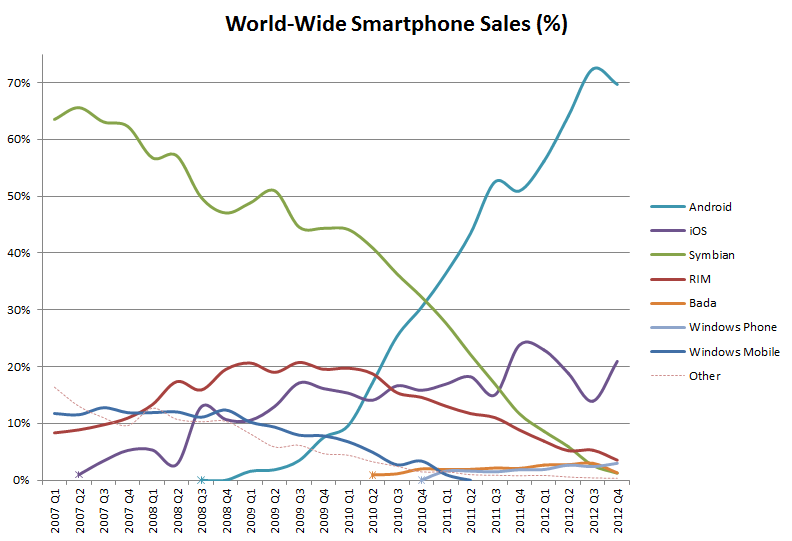
\includegraphics[width=0.8\columnwidth]{figs/World_Wide_Smartphone_Sales_Share}
\caption{Worldwide Market Share of various mobile OSs - from \citep{wikimobileshare} and \citep{gartnerq42012}}
\label{fig:mobileshares}
\end{center}
\end{figure}


Mobile OSs, like the PC operating systems of the 1990s, have a few major players that wield the most influence, as seen in Figure \ref{fig:mobileshares}. The two largest operating systems in the mobile area are Android and iOS. Apple's iOS, made exclusively for the Apple iPhone and iPad, runs on over 20\%\citep{gartnerq42012} of all smartphones globally, as of the end of 2012. Google's Android, released as an open source OS, has many different hardware manufacturers: Samsung, LG, HTC, Motorola, and many more. It currently runs the majority of smartphones globally, with 70\%\citep{gartnerq42012}  marketshare. Some of the less popular though still significant mobile operating systems are Windows Phone, with 3\%, and Blackberry, with 3.5\%\citep{gartnerq42012} . 

\subsection{iOS}
Apple released the iPhone in 2007. ``Entry into mobile phones might have been a risky move for Apple. The industry was dominated by Nokia, Motorola, and Samsung, with roughly 60\% market share''\citep{yoffie2010apple}. However, ``the Apple iPhone was a huge success. Considered by Time magazine the invention of the year 2007 ... it completely changed the mobile phones industry dynamics''\citep{reis2012leadership}. Apple's iPhone and iOS were novel due to their touch friendly and intuitive OS, as well as their digital distribution platform, the App Store\citep{yoffie2010apple}. In 2012, Apple sold over 130 million iOS devices\citep{gartnerq42012}.

\begin{figure}[h]
\begin{center}
%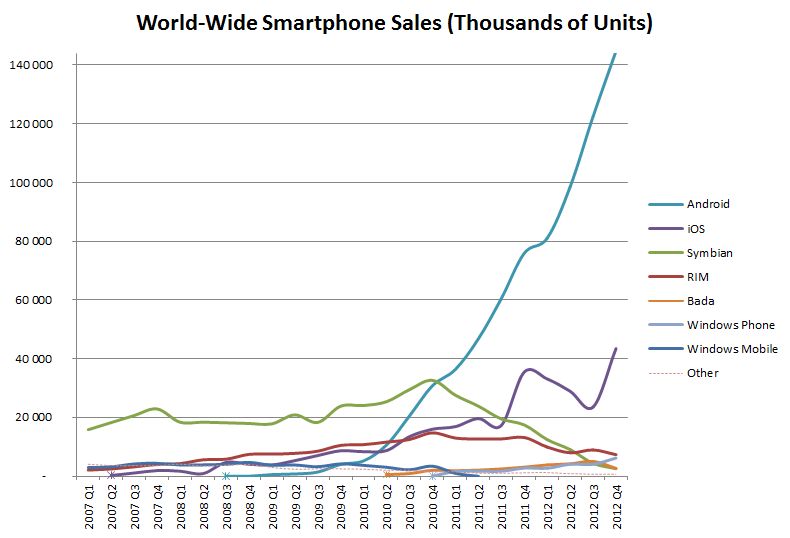
\includegraphics[width=0.8\columnwidth]{figs/World_Wide_Smartphone_Sales}
\caption{Worldwide Sales of various mobile OSs - from \citep{wikimobilesales} and \citep{gartnerq42012}}
\label{fig:mobilesales}
\end{center}
\end{figure}


\subsection{Android}
Started in 2003 by Andy Rubin and Android Inc (previously the makers of the T-Mobile Sidekick), Android was acquired by Google Inc. in 2005\citep{businessweek2005}. ``Android was built from the ground-up to enable developers to create compelling mobile applications that take full advantage of all a handset has to offer. It was built to be truly open. For example, an application can call upon any of the phone's core functionality such as making calls, sending text messages, or using the camera, allowing developers to create richer and more cohesive experiences for users''\citep{ohaandroidoverview}. Since its initial release in 2007\citep{oharelease2007}, Android has sky-rocketed to the most used mobile OS in the world, with over 70\% marketshare, and 144 million Android devices being sold in Q4 of 2012 alone\citep{gartnerq42012} --- more than Apple had the entire year, as seen in Figure \ref{fig:mobilesales}.



\subsection{Goals of Mobile OSs}
All these mobile OSs share many common goals and challenges. The diversity of hardware that smartphones were designed to replace, along with other constraints and features, requires a mobile OS that's designed from the ground-up to deal with many different challenges than the typical PC OS. Some of the main design challenges for a mobile OS include: 
\begin{itemize}

\item Small memory footprint, battery-conscious, and other resource restrictions

\item Access to a wide variety of personally identifiable information (PII)

\item Access to a wide array of hardware

\end{itemize}
In order to effectively enforce rules on battery consumption, low-latency UI, and personally identifiable information, a new security model was created, centered around the concept of the \textit{App}. 


%To understand the nature of modern mobile malware, we first examine the context. The two main models, that of iOS and Android, are compared and contrasted here.

\subsection{The \textit{App} and Sandboxing}

In the mobile world, \textit{Apps} are isolated and sandboxed programs, generally designed with a singular purpose. They lack dependencies and generally less privileged than system software for performing many tasks. The mechanisms for accessing functionality outside of their sandbox is enforced by a set of policies the system holds, specific to that app. On some platforms, like iOS, only one app may run at any given time, and background computation is virtually non-existent (with some exceptions\footnote{Minor amounts of computation can be done to compute background audio, and other isolated background tasks.}), along with many other restrictions. On Android and other mobile platforms, many more features are available to apps, but in all cases, the app lifecycle is well-defined and controlled by the system much more than on a PC OS.

Various reasons exist for the tight sandboxing of mobile apps. Power and resource consumption are certainly a factor --- mobile OSs generally reserve the right to terminate apps if they attempt to allocate too much memory. Controlling access to hardware also helps with this --- allowing apps to keep the phone awake could easily drain battery. However, another reason for sandboxing, and arguably more important, is protecting Personally Identifiable Information.

\subsubsection{Personally Identifiable Information}

Personally Identifiable Information (PII), as defined by the National Institute of Standards and Technology, is ``any information about an individual maintained by an agency, including (1) any information that can be used to distinguish or trace an individual's identity... and (2) any other information that is linked or linkable to an individual'' \citep{mccallister2010guide}. Mobile devices --- having blended cameras, cell phones, GPS devices, and PCs into one device --- have an extremely diverse amount of PII, including phone numbers, contacts, location history, bank account numbers and pictures. For many of these datasets, mobile OSs actually organize them into databases with the intention of allowing third parties access to them. Contact lists, SMS, photographs and location history are available to apps on virtually every mobile platform in some official way. This is a driving motivation for a greatly improved security model for mobile OSs: controlling third party software's access to PII. 

% Expand more on this.

\subsubsection{Digital Distribution Platform}

The final major difference between mobile OSs and PC OSs is the distribution of code. No mobile OS allows third party code to be run outside of the sandbox, and all of them require the user's consent before installing an app. All apps must be signed. In general, there is one main distribution channel for all apps on a mobile OS. This tightly-controlled distribution both aids in security, and controls the ecosystem around that mobile OS.

\subsubsection{Apple's App Store}
The first major digital distribution platform for mobile apps was Apple's App Store\citep{AppleAppStore}. Its model has been repeated by almost all major mobile app distribution platforms. The basic premise is simple: developers sign up to the app store, pay a fee (usually yearly), and submit fully-finished apps. A reviewer runs the app in a monitored sandbox, watches for unusual behavior, checks for stability and usability, and approves it. Once the app has been approved, it is released onto the app store, at which point anyone can download it. The approval process, as well as the high monetary fee, act as a way to ensure only safe and high-quality apps are available for that platform. In this type of platform, typically no apps may be installed from other sources. On iOS, initially this was the main method of security: if the app passed the inspection, it was acknowledged as safe and virtually unmonitored unless someone noticed something unusual and reported it. However, in recent years, after certain incidents (see section \ref{sec:path}), apps must still request permission from the user to perform certain tasks.

\subsubsection{Android Permissions}
Android's distribution platform takes a different approach. At its core is Android's security model: The Permission System (see section \ref{sec:permissions}). When Android Apps are packaged, they declare what capabilities they will use and the user reviews them before installation. If the user approves the app, it may use the requested capabilities at any time: little restrictions are placed otherwise. With this barrier in mind, the Google Play Store (formerly known as the Android Market), or GPStore, opts for an alternate model to iOS, in which the developer pays a smaller fee and apps do not go through a formal approval process. After an app's submission, it is immediately released to the public for users to download and run. Android assumes that the metadata the GPStore provides --- App Name, Developer Name, Description, Reviews, and Ratings --- are enough for the user to determine if the app should be trusted with the permission set it is given (see Figure \ref{fig:gpstoreapps}). In fact, Android even allows the device to accept apps from third party sources --- a practice known as \textit{sideloading} --- although it is disabled by default. This has spawned a large number of third party app sources, all of which rely on the Permission system for user protection.

%GPSTORE IMAGE AND CHART EXPLAINING THE LETTERS.

\begin{figure}[h]
\begin{center}
%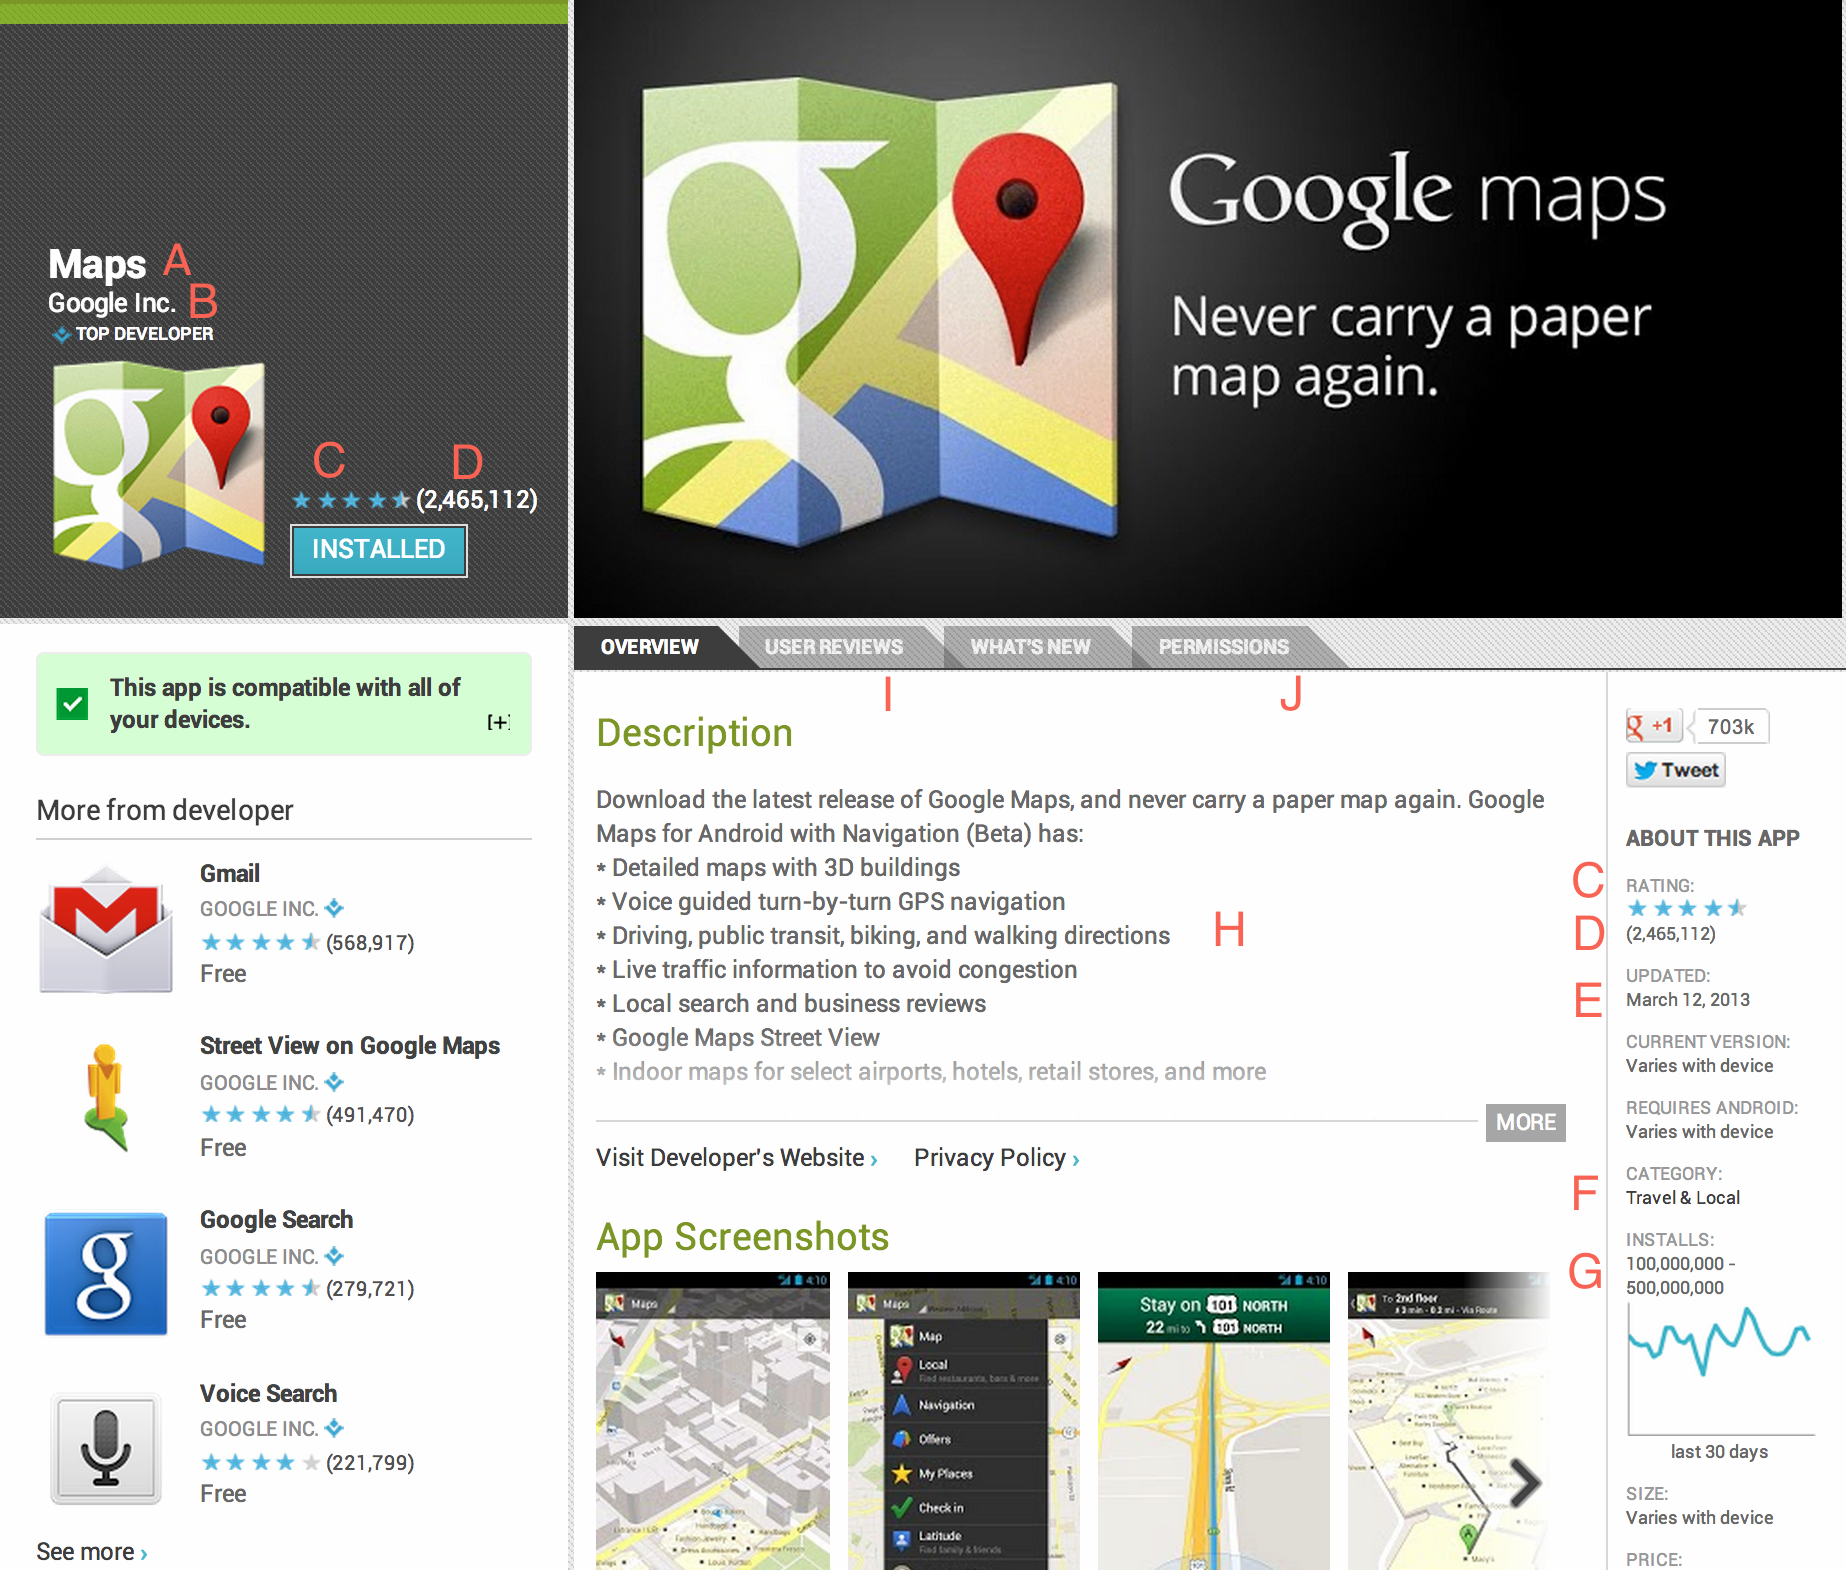
\includegraphics[width=0.9\columnwidth]{figs/GPStoreAppPage}
\caption{A sample page on the Google Play Store, see \ref{tab:gpstorekey}}
\label{fig:gpstoreapps}
\end{center}
\end{figure}

\begin{table*}[h]
\begin{small}
\begin{tabular}{l|l}

\textit{A} & App name  \\
\textit{B} & Developer Name  \\
\textit{C} & App Rating  \\
\textit{D} & Number of ratings  \\
\textit{E} & Date the app was last updated  \\
\textit{F} & Category in the Google Play Store it falls under  \\
\textit{G} & Number of installs (range, not exact number)  \\
\textit{H} & Description of the app  \\
\textit{I} & Reviews of the app  \\
\textit{J} & Permissions the app requests  \\

\end{tabular}
\end{small}
%\vspace{-0.2in}
\caption{Various properties of a Google Play Store app page}
\label{tab:gpstorekey}
%\vspace{-0.1in}
\end{table*}

%The core concept behind Android security - Permissions - are a static contract of capabilities. However, in this paper we propose an alternate means of conceptualizing security, which focuses on the interrelationship between the user's perception of the app, and the app's actual behavior. We call this the ``user-app agreement'', and will elaborate on it more later. 

\subsection{Mobile Malware}
Malware, as defined by the US Department of Homeland Security, is ``short for malicious software. Programming (code, scripts, active content, and other software) designed to disrupt or deny operation, gather information that leads to loss of privacy or exploitation, gain unauthorized access to system resources, and other abusive behavior'' \citep{nash2005undirected}. Like PC OSs, malware is present on mobile OSs, although there are differences.


The tighter security model of mobile OSs has a notable effect on mobile malware. With tight control in sandboxing and app distribution, the usual viruses, trojans, and other exploits are more difficult to employ. The main vectors are either OS-level exploits --- sneaking past the app review process --- or through sideloading of apps. When looking at the two main mobile OSs, a stark contrast is shown. iOS has had  \textit{jailbreaking} --- privilege escalation exploits --- dating back from its first release \citep{damopoulos2011isam}. Alternately, the first Android exploit was not discussed until 2010 by security researchers Papathanasiou and Percoco \citep{papathanasiou2010not}, and was not seen in use until early 2011\citep{castillo2010android}. On the contrary, no sideloading is possible for iOS, and there have been very few instances of malware sneaking past Apple's App Store review process (although it has happened\footnote{In July 2012, SecureList noticed an iOS app that uploaded all of the user's contacts to a remote location without their consent\citep{SecureList2012}, but others argued this was not as devious as made out to be\citep{trendmicroios2012} }). With 95\% of all mobile malware\citep{nq2013}, Android's malware situation is a product of the sideloading and lack of review process found in GPStore\citep{nq2013}. %Of all the mobile malware found for iOS and Android, over \temp{some percent} used no system-exploits at all, \temp{some percent} on the main app distribution platform.

 On mobile devices, one of the dominant goals of malware is to gather information that leads to loss of privacy, found in over 28\% of mobile malware in 2012 alone\citep{nq2013}. The trend of malware possessing no system exploits, but gathering information that leads to loss of privacy --- Info Theft Malware --- is one that Android's Permission-based security model is ill-equipped to handle. Android's permission system relies on the user to determine upon installation if a list of capabilities should be entrusted with the given app. The user is not given a say in how or when the capabilities may be used, nor the ability to reject specific capabilities. At the same time, the mechanisms that keep mobile OSs safe are forcing malware writers to use more subtle techniques, often without exploits. This all works against the user.

This paper attempts to address this key issue through various means. We first introduce several novel concepts for analyzing apps and malware on Android. We then analyze the state of Android apps and Permissions with the most comprehensive Android app database available, Android Census. Finally, we propose several novel improvements to the Android security architecture, called AndroMEDA, aimed at expanding on of our conceptual work.





















\section{Related Works}

\subsection{Android Extensions}
AndroMEDA is far from the first to attempt to address the issue of malware on Android. As early as 2009, frameworks such as SAINT\citep{ongtang2012semantically} built off of the Android Permission Framework by implementing runtime policies the user could define per app. Later on, projects like TISSA\citep{zhou2011taming} built off of SAINT by implementing varying levels of obfuscated data. When an app running on TISSA requests access to the contacts database, TISSA can either provide the app with the full database, a limited portion, an anonymized portion, or no information. Not all PII was covered in their framework, nor were any temporal rules established: the system behavior for a specific database of PII for an app was consistent across requests. These events were not shown to the user either, unlike TaintDroid\citep{enck2010taintdroid}.

TaintDroid is a novel extension for Android, focused on flow detection of PII. By modifying the low-level VM of Android --- Dalvik --- variables are tainted once they access PII. This taint flows throughout the system, and when the variable reaches a designated exit location, the event is logged and alerted to the user. Finally, YAASE\citep{russello2011yaase} is a relatively new security extension, but combines many aspects of TaintDroid and TISSA to become an extremely powerful way of detecting information flow and prevention.

There are several main shortcomings in all of these frameworks. First off, they all require significant modification of the Android codebase, thus creating very difficult work for developers who seek to incorporate these extensions into their Android OS. Performance impact, although by many accounts is somewhat negligible, certainly plays a role in a decision to incorporate such security extensions.

Second, the complex rulesets required build off of the Permission Framework, adding additional rules the user may configure. However, a study by Berkeley suggests only 17\% of users paid attention to permissions at install time, and only 3\% correctly remembered them later\citep{felt2012android}. Clearly, tasking the user with more work is the wrong approach. Looking at malware through the context of the UAA, all but TaintDroid fall short in one key regard: alerting the user of suspicious behavior.

Several frameworks have touched upon the concept of the UAA. Andromaly\citep{shabtai2012andromaly} (developed in 2010), pBMDS\citep{xie2010pbmds}, and Crowdroid\citep{burguera2011crowdroid} all attempt to classify malware based upon its interaction with the user. However, none actually ask immediate input from the user --- a fundamental flaw that limits the ability to adapt to the user's specific UAAs.

\subsection{Android Sandboxes}
On the other side of malware detection is \textit{automated} malware detection. The major project in this regard is Google's Bouncer\citep{googlebouncer}. Introduced in 2011, Google Bouncer is a system that runs malware in a highly-observed sandbox, and watches for suspicious behavior. Since its release, it has been highly criticized\citep{mansfield2012android}, with researchers finding over twenty ways to circumvent it.

Similarly, TrendMicro provides its solution, App Reputation\citep{trendmicroappreputation}. It runs apps in a ``cloud'' sandbox, watching for connections to suspicious websites, as well as other monitoring. A research project, Paranoid Android\citep{portokalidis2010paranoid}, runs in a similar vein, monitoring apps in a sandboxed Android OS. However, in order to get accurate information on app behavior, actions must be recorded.

Most all of the frameworks listed above, however, especially the sandbox tools, assume a clear ruleset to be established classifying malicious behavior versus benign behavior. They require a clear line to establish what constitutes trusted behavior versus untrusted. Unfortunately, this counters the concept of the UAA, in which every individual action has a complex set of rules that result in an acceptable behavior versus unacceptable. Users may also have vastly different rules for what constitutes malicious behavior. Apps that send the Unique Device ID (UDID) and location information to ad networks might seem malicious to some users, and perfectly normal to others.


\subsection{Android Surveys}

%\subsection{Conclusion}
%This should be the actual conclusion
%The main counter argument to all of these frameworks is the example of SoundComber: it records audio in the background, looking for PII. Some frameworks and policies may immediately flag this as malware; but one can conceive of perfectly benign apps that follow this exact same formula: dictation apps that transcribe speech to text over long portions of time, audio broadcasting utilities, etcetera. Apps that take all PII and upload it to a server may be classic malware --- or simply a backup utility. Context and use --- and more generally the UAA --- are an extremely important part of malware detection that's missing from modern Android security frameworks.
\subsection{Contribution}
WE DUN STUFF.





















\section{Concept}
\subsection{Mobile Threat Model}
Apps can steal PII undetected. Like Soundcomber.

Malware on mobile devices has seen a departure from past exploits. The wealth of Personally Identifiable Information easily available on mobile OSs increasingly makes them the focus of malicious software. In addition, the tight sandboxing constraints often forces malware writers to either find exploits to break out of the sandbox or to write malware that cloaks itself as benign. Without finding exploits, code can not be run by the user unless it is in it is form and comes through a trusted channel (unless of course that security feature has been disabled). Once on the device, malware has several main methods of attack.

\subsection{Installation}
The three primary ways in which malware can be installed on an Android device are \textit{Repackaging}, \textit{Update Attack}, and \textit{Drive-by Download}\citep{zhou2012dissecting}. The first two are designed to sneak malware into the Google Play Store or other third party stores; and the third is designed to trick the user into installing it by mistake. \textit{Repackaging} deals with the technique of taking an existing app, adding malicious code to it, and repackaging it again (discussed further in Chapter \ref{sec:incognitoware}). \textit{Update Attacks} typically build off of \textit{Repackaging}, but do not acquire malicious code until later, making static detection difficult\citep{zhou2012dissecting}. The last, \textit{Drive-By Downloads}, is often tied with \textit{Repackaging}, but is not presented in an official app channel. Instead, it is downloaded when the user visits a webpage or clicks a link\citep{zhou2012dissecting} and Android prompts the user as to whether or not they would like to install the app. All three methods involve concealing the intent of the malware and passing as a legitimate app; they do not use browser exploits or system exploits to install the initial malware without the user's consent.

\subsection{Malicious Actions}
Once installed on the device, Android malware has several main methods of attack. Xuxian Jiang
 and Yajin Zhou\citep{zhou2012dissecting}, along with Spreitzenbarth\citep{spreitzenbarth2013}, and Hackmageddon\citep{hackmageddon2011} define four major categories: \textit{Privilege Escalation Attack}, \textit{Remote Control Attack}, \textit{Monetary Service Attacks}, and \textit{Privacy Info Theft}. 


\subsection{Privilege Escalation Attack}
\textit{Privilege escalation attacks} take several forms on Android. The basic premise is simple: acquire access to operations beyond what the sandbox and granted capabilities provide. The main way to accomplish this is via \textit{rooting}.

\subsubsection{Rooting}
\textit{Rooting} is the act of acquiring root --- or administrative privileges --- on an OS. Typically mobile OSs do not provide the user or apps with root capabilities and instead reserve that for a set of trusted system processes. However, by finding vulnerabilities in these services or exploiting the OS itself, apps can escape the sandbox. After an app has been granted root capabilities, the permission system no longer applies to it: it can simply access whatever it wants. These attacks are difficult for the system to detect as all monitoring of apps relies on monitoring the sandbox --- there is no way to track an app that escapes the sandbox. This technique is commonly employed by botnets, giving remote access to the core system. 

Many examples of root exploits exist, dating back to 2011 with \textit{RageAgainstTheCage}\citep{droiddream}. These root exploits were very popular for non-malicious purposes, circumventing the device's sandbox to install a permanent root binary, creating a similar setup to a typical UNIX computer, where root may be acquired after a password and/or permission. In March 2011, however, DroidDream was discovered. DroidDream used \textit{RageAgainstTheCage} to silently install additional applications in the background, stealing PII and forming a botnet. By the time Google remotely removed it from the market, it had been downloaded an estimated 50,000 to 200,000 times\citep{castillo2010android}, which was the largest bulk-remote-removal of apps seen from the GPStore. From then on, a stream of root exploit malware was found based off of exploits such as \textit{RageAgainstTheCage}, \textit{udev}, and another called \textit{GingerMaster}\citep{gingermaster}.

\subsubsection{Recent Android Rootkits}
\label{sec:recentrootkits}
\textit{GingerMaster}\citep{cskills2011} is significant because it is the last known root exploit malware seen in use. Designed for Android 2.3.3, it can currently run on 45\% of all Android devices in use, according to the official Android Dashboard\citep{androiddashboard}. In reality, however, of that 45\%, almost all have been patched to fix the exploit\citep{cskills2011}. All previous exploits were patched in Android 2.3\citep{cskills2011}, meaning less than 6\% of all active Android devices are vulnerable to them. Since Android 4.0, Google has focused greatly on security, improving ASLR\citep{threatpost2012} and hardening system services\citep{androidjbsecurity}. No known rootkits exist --- malicious or not --- for Android 4.0 and up comprising 54\% of active Android devices.

 %Several exploits became very popular for malware writers, starting with DroidDream in 2010 <cite>, then RageAgainstTheCage, PSNeuter, and GingerBreak. When DroidDream was first discovered, it was downloaded over <50,000> times in the GPStore - prompting the largest bulk-remote-removal of apps Google has ever been discovered to have performed. However, most of these attacks have been fixed by vendors as of Android 2.3.3 - meaning the total amount of current devices in use that are vulnerable to these bugs being roughly <10%>. After these attacks, Android has taken definite steps to up its security. Since 4.0, proper ASLR has been implemented, as well as other security enhancements. There has been no known malware written for Android 4.0 and up - over <50%> of the active market.

\subsubsection{Confused Deputy Attack}
The second main vector for privilege escalation attacks is the \textit{confused deputy attack}\citep{hardy1988confused}. In this scenario, services that guard sensitive operations are ``tricked'' into performing them. For example, if a Content Provider forgets to check a permission, or if a developer finds APIs that do not correctly perform a permission check. Perhaps the simplest example of this is the ability for any Android app to contact remote servers by asking the web browser to open a URL. By including sensitive data in the URL, an app may still transmit sensitive data to a remote server without ever requesting the \textit{INTERNET} permission. Projects like XManDroid\citep{bugiel2011xmandroid} and Quire\citep{dietz2011quire} address this by extending Android to analyze inter-app communication and detect this kind of attack. %Despite all of these concerns, it is worth noting that no known malware has been used to exploit this. 

\subsection{Remote Control Attack}
\textit{Remote Control Attacks}, frequently called \textit{botnets}, are the ability for malware to accept commands from a remote server, controlling the device. This technique is common --- Xuxian Jiang
 and Yajin Zhou\citep{zhou2012dissecting} found in 93\% of Android malware --- and is often used in conjunction with other attacks\citep{spreitzenbarth2013}.

\subsection{Monetary Service Attack}
\label{sec:premiumsms}
The second malware technique is possibly the simplest: perform services on behalf of the user that cost money. Examples of this include calling costly phone numbers and sending premium SMS messages. Typically these actions are performed without notifying the user, and are only visible after the user checks their bill. These attacks have been prevalent in the Android market for quite a while, with NQ Mobile\citep{nq2013} listing it as one of the top three threats of 2012, and being found in 39 of 119 of the malware documented by Spreitzenbarth\citep{spreitzenbarth2013}. However, recent versions of Android (after 4.2 Jelly Bean\citep{androidjbsecurity}) have taken the step of warning the user before premium SMSs are sent. %This attack vector, while common, will see a reduction in the future thanks to these measures.

A prime example of this is FakeInst\citep{avastfakeinst}, a repackaged version of Instagram\citep{instagramandroid} that sent premium SMS messages on start. ``In the background, the fake downloader sends a premium rate SMS to the number based on the country of origin for the user''\citep{avastfakeinst}. In many cases, the premium SMS messages would end up being billed to the user for over \$4 each\citep{avastfakeinst}, without ever alerting the user. Messages are often deleted by the app, removing the trace until the user gets their bill.
%\temp{Expand on this more}
%show some examples of this. expand on this more.

\subsection{Private Info Theft}
The last malware technique is the most significant, and represents the largest departure from typical malware: apps that steal PII, or \textit{Info Theft Malware}. The theme is fairly straightforward: provide the user with a seemingly legitimate app, but in the background acquire large amounts of valuable data --- including call logs, contacts, and photos --- and send them to a remote server. This fits with the main themes of mobile computing: the consolidation of many sources of PII all in one device. 
%However, this is the biggest departure from typical malware. 
To the system no unusual operations are performed and no exploits are ran. The qualification for Info Theft Malware lies in the ``use'' versus ``misuse'' of PII; often times, this line is blurred.

\subsubsection{Path on iOS}
\label{sec:path}
A large distinction of what constitutes as privacy malware to an individual stems from the user's expectations of how the app will use their PII. Consider the case of the Path iPhone app, which in February 2012 was discovered to be uploading the user's entire contact list to Path's servers, without any consent from the user\citep{thampi2012}. It is fairly uncontroversial for a social network to read your contact data, and the act of scanning contacts to help ``find your friends'' on Path wasn't out of the ordinary. As VentureBeat discovered: ``Facebook, Twitter, Instagram, Foursquare, Foodspotting, Yelp, and Gowalla are among a smattering of iOS applications that have been sending the actual names, email addresses and/or phone numbers from your device's internal address book to their servers''\citep{vb2012addressbook}. Ultimately, however, the outrage was sparked because of how unexpected the behavior was.

The Path incident sparked several key changes in iOS's security model: having a popup occur when an app requests access to the contacts database and allowing the user to reject the request. This, in general, is a one-time request, after which the app is granted unrestricted access to the content\citep{AppleContacts}. This change, however, did not fully address situations like Path, in which is was less about the app simply having access to the data, and more about what the app actually did with the data behind the scenes. When these actions did not match up with user expectations, the app was treated as malware until the situation was cleared up by Path. The next day, Path issued an update that immediately explained to the user what they were going to do with the data and why.

It is worth noting that the only reason Path's contacts upload mechanism was discovered was by accident: Arun Thampi discovered it as part of a company hackathon, and only via sniffing the HTTP requests coming from the phone. An ordinary smartphone user would not have access to these tools, nor have the time and patience to sift through the data to spot unusual behavior. These actions are unchecked and hidden from the user, denying them the ability to decide for themselves if they are comfortable with them --- supporting our motivation for AndroMEDA.

\subsection{User-App Agreement}
The Path incident, however, lies at the heart of mobile malware: misuse of PII lies in the abstract definition of how the app is expected to behave. Apps that violate this expectation of behavior are classified as malware, while apps that do follow this expectation are not. This agreement between the user and the app --- the User-App Agreement (or UAA) --- is an informal understanding the user has as to what actions an app will take. This differs from the Permission Fingerprint, which is a measure of what actions the app is capable of performing, dealing instead with exactly when and how those actions are taken. Since this agreement is not formally defined, it is acquired through external trust in an app. This happens in various ways, through the description the app provides, the knowledge and referral of the app from other trusted sources, or the trust in the developer. The UAA is not a measure of how trustworthy an app is, but rather a framework for the user consenting and trusting specific actions an app may take.

\subsubsection{UAA Example - Social Networking App}
An example of UAA can be seen in the expected behavior of a hypothetical app and user. The first is a large Social Networking app, which requests permission to access internet, send SMS messages, and read the contacts database. If the Social Networking app accesses contacts when the user requests ``find my friends'', and it sends SMS messages after the user messages another user who is not ``online'', these actions fall within the UAA of the Social Networking app and the user. However, if the contacts database is read and uploaded to a remote server without the consent of the user, this may violate the UAA and break the trust of the user (expanding on the example of Path). 

\subsubsection{UAA Example - Social Game}
The other example is a little known developer's game, which, like the social networking app, also requests permission to access internet, send SMS messages, and read contacts. These documented capabilities in the Permission Fingerprint may be enough to violate the UAA: the user may not trust an app with the capability of these actions. However, in the case that the user does, or simply doesn't pay attention, the app still may not violate the UAA. If the app is an online game and asks you to find other people you know who are playing it, this would more likely than not violate the UAA. Furthermore, if it sends SMS messages to your friends telling them to download the game, this would breech the UAA and break the trust of the user.

In both examples, the apps have the exact same Permission Fingerprint, but vary widely in their expected behavior, and which actions are trusted and untrusted. This misuse of PII and other device capabilities fits with our definition of malware, and highlights the shortcomings of the Permissions framework: being unable to deal with the subtle differences between trusted behavior and untrusted behavior. Indeed, every user may have a very different understanding of what acceptable behavior is. Therefore, UAA plays a crucial role in classifying apps in relation to Info Theft Malware.

\subsection{Proof of Concept Malware in Academia}
In the realm of malware research in academia, several prominent proof-of-concept examples further demonstrate the vague line between use and misuse of PII and our concept, the User-App Agreement. The most notable one is SoundComber\citep{schlegel2011soundcomber}. It passes off as a benign app, but, in the background records audio and does on-phone processing to find sensitive PII, after which it uploads the information to a remote server. This app is unique because of its simple Permission Fingerprint, as well as its ability to gather sensitive PII from a channel not suspected to be very rich in PII.

The second prominent example of academic malware on Android is TapLogger\citep{xu2012taplogger}. TapLogger imitates a simple touch-based game, learning the vibration patterns of the device for each tap. By recording the vibration patterns in the background, it attempts to discover passwords and other sensitive keyboard events, all through a seemingly trusted sensor. TapLogger requests no Permissions; therefore its behavior is possible for any app. 

In Chapter \ref{sec:incognitoware}, we expand upon these examples to present an additional dataset of IncognitoWare -- repackaged apps with malicious software added --- designed for research purposes. We keep the Permission Fingerprints identical to the cloned app, making detection exceptionally difficult. 
%reference future malware set

\subsection{Conclusion}
The landscape of malware on Android follows many clear patterns. The first is the use of masquerading as benign apps, and passing through trusted or semi-trusted channels to enter the device. Once on the device, the malware manifests itself as one of four main categories of attacks --- privilege escalation attacks, remote-control attacks, monetary service attacks, and personal info theft. Of these categories, privilege escalation attacks and monetary service attacks are the easiest to protect against --- and indeed Android has taken serious steps to mitigate these. The third time of attack, however, personal info theft is the most difficult to mitigate on Android due to the shortcomings of the Permissions framework, and the wide spectrum of severity these attacks can take. Since these attacks may vary in interpretation per user and lay in the subtle communication between the user and the app, we highlight the need for a concise representation UAA, where the user can evaluate the actions themselves.


\subsection{System Goals}
Provide feedback to the user, allowing them to identitify misuse of PII. Of the attacks described above, the only ones we care about are PII attacks.































\section{AndroMEDA Framework}
\subsection{Overview}
Android Malware Evaluation Detection and Analysis (AndroMEDA) is designed to complement existing Android security extensions like TISSA\citep{zhou2011taming}, TaintDroid\citep{enck2010taintdroid}, YAASE\citep{russello2011yaase}, and XManDroid\citep{bugiel2011xmandroid}. The goal in building AndroMEDA was making the minimal amount of changes to the Android system in order to extract sufficient amounts of information. Portability was important, as code that is easier to port can be more easily adopted. Along with being lightweight and fast, portability further forced the extension to be as simple as possible. The framework aimed to be as independent of hardware as possible, with the ability to work on any device: smartphone, tablet, TV, or future devices like Google Glass. This portability meant as few changes to the low-level drivers and kernel as possible.

Functionally, the main goals of the framework are to better understand how apps behave, what PII and capabilities they access, and to provide the user with the information necessary to quickly evaluate an app's actions in relation to its UAA. Logging sensitive events, finding strategic opportunities to expose these events to the user, giving the user actions to perform in reaction, are key steps in mitigating malware --- especially Info Theft Malware --- on Android. Unfortunately, as discussed in Chapter \ref{sec:permissionrejection}, Android does not log these sensitive events natively, thus motivating this framework. Ultimately, it is expected that a framework such as this would not eliminate malware on Android, but rather be part of a larger system.

As a base for our framework, we chose CyanogenMod\citep{cyanogenmod}, a third party open source Android distribution created by volunteers. It provides firmware for a wide variety of Android devices, and its user-base is comprised of people seeking to replace their stock OS. This makes it an ideal candidate to fork our framework from --- our changes can therefore be incorporated into the over 4.1m+ installs of CyanogenMod\citep{cyanogenmodstats}.

\subsection{Details}
Android, as an open source project, is hosted at \url{source.android.com}\citep{androidsource}, as a series of \textit{Git} repositories managed by a meta-script called \textit{repo}. Its source tree is organized by project type; ``frameworks'', ``external'' and ``libcore'' are the top-level folders we focus on. ``Frameworks'' contains all of the Java, C++, C, assembly code, and other code that compose the core framework that runs on top of the main libraries. ``Libcore'' and parts of ``external'' comprise the main libraries. The bulk of the code lies in ``frameworks/base''.

%maybe add more?

\begin{figure}[t]
\begin{center}
%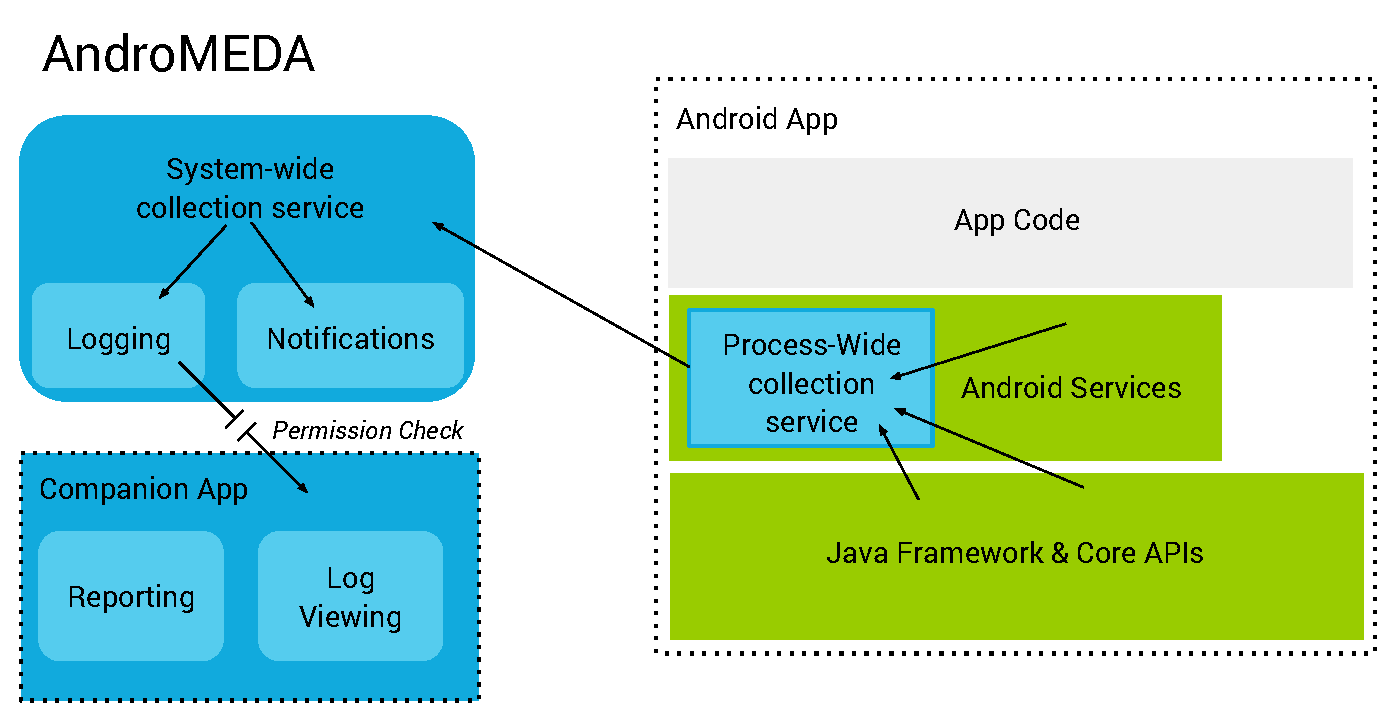
\includegraphics[width=1.0\columnwidth]{figs/AndroMEDA-Architecture-Overview}
\caption{AndroMEDA Architecture Overview}
\label{fig:andromedaoverview}
\end{center}
\end{figure}

The architecture (seen in Figure \ref{fig:andromedaoverview}), is organized into two main parts: (1) a collection of hooks in the API and (2) a system service to collect this information. The collection of hooks in the API calls into a process-wide service that translates them into events that get sent to the global system service. At the start of every new Dalvik process, the process-wide collector installs hooks into the framework that notifies the collector when the APIs are called.

\subsubsection{System Extension}
\begin{figure}[t]
\begin{center}
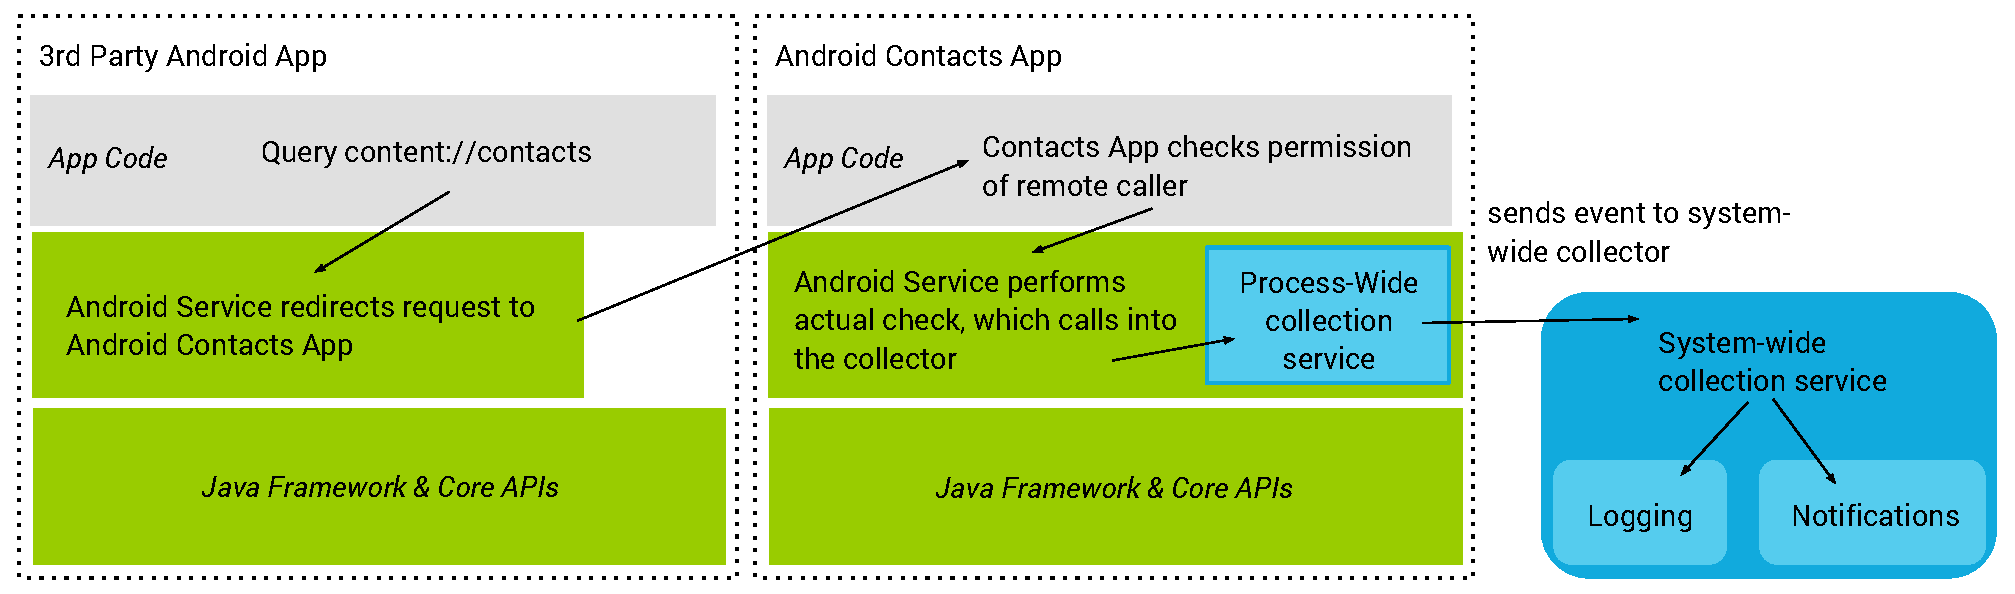
\includegraphics[width=1.0\columnwidth]{figs/AndroMEDA-Inter-App-Example}
\caption{Example code path of an app requesting data from the Contacts app}
\label{fig:interapp-example}
\end{center}
\end{figure}

The hooking mechanisms vary depending on the exact call being instrumented. Android has a standard mechanism for checking permissions in many cases; and we placed a hook where this is enforced. Usually, this occurs during a Remote Procedure Call (RPC) with the process that owns the data; as such, the remote UID is sent along (as seen in Figure \ref{fig:interapp-example}). Unfortunately, many permissions are not checked through this method, but Android Permissions Demystified\citep{felt2011android} has a comprehensive list of API calls and the permissions they require, making it easy to locate essential APIs to instrument. For the more difficult APIs, a static global callback variable is placed in every class we want to instrument. Upon launching the process, our local collector populates these global variables with callbacks that marshal the data to the main collection service. Calls are then made to the callback at the appropriate times in the API's normal function (seen in Figure \ref{fig:camera-example}). Using this method, we are able to instrument any API call, getting more data than when the permission is simply checked.

\begin{figure}[t]
\begin{center}
%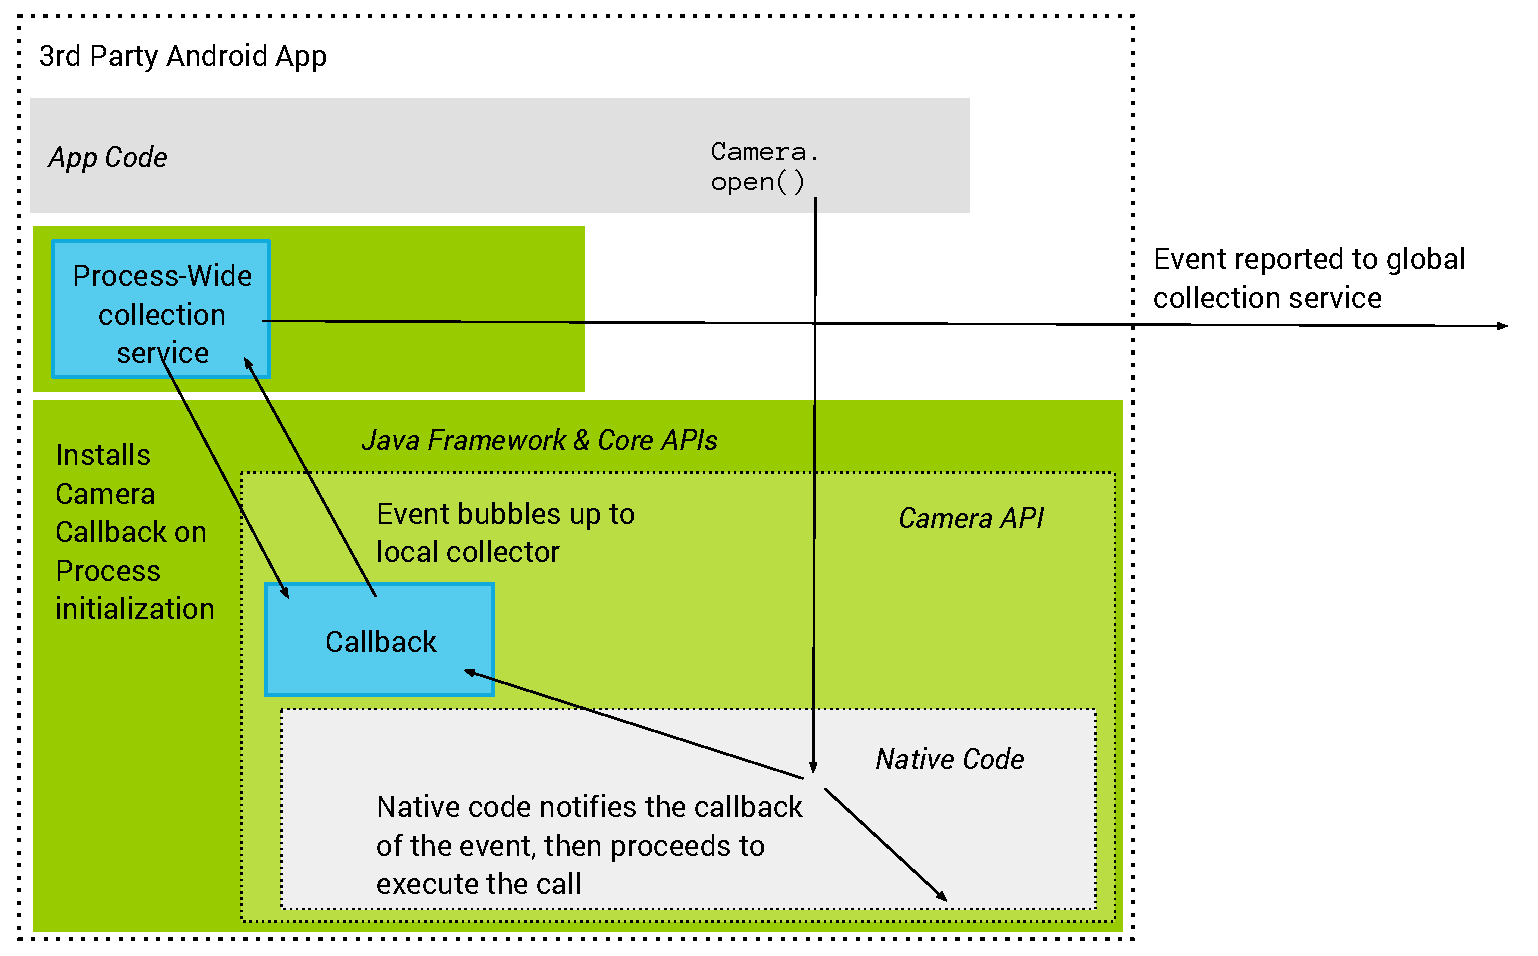
\includegraphics[width=1.0\columnwidth]{figs/AndroMEDA-Static-Example}
\caption{Example code path of instrumenting the Camera API}
\label{fig:camera-example}
\end{center}
\end{figure}

For C and C++ level code, we establish hooks in the Java Native Interface (JNI) --- Java's method of communicating with native code --- to call back to the main object. Since using JNI to call back into Java from C is cumbersome and error prone, the hooks call into a local callback, which then calls the process-wide callback accordingly. An example can be seen in Figure \ref{fig:camera-example}.

The ability to log virtually any API call is extremely valuable. Not only are permission events logged, but more fine-grained events --- like the starting and stopping of an audio recording --- can be measured. Internet sockets are logged, along with all POST data set out. Not only is this system light-weight and fast, but it does so with as little modifications as possible. No kernel-level or Dalvik-vm-level changes are required.

The global service acts as the central point of collection of all events. It runs in its own process and uses Binders (Android's RPC) to communicate with other processes, which feed events into it. These calls are asynchronous, and do not block the remote caller. The service is responsible for logging and processing the events, as well as taking action on them.

Two way communication is also possible. An app's local collector can query the global service and acquire a list of events for a given package (among other things). This allows user-level apps to be written to leverage AndroMEDAs findings.

\subsubsection{Companion App}
We wrote a companion app to allow the user to inspect the information being gathered by AndroMEDA. The companion app responds to the Intents broadcast by the notifications that AndroMEDA displays to the user. This reports a log of events by that app and allows the user to take action. The user may report an app or uninstall it. A simple web service was set up to aggregate these reports.

The companion app is significant because it does not require the AndroMEDA framework to be present on the phone to function. Despite the unavailability of local logs, the companion app can still query the web service, and view event histories that other users have published.





























\section{Analysis}





























\section{Evaluation}

With AndroMEDA, we attempt to build on top of the Android Permission system, to do a better job of enforcing the User-App Agreement. The main reasons why the Permission System failed to differentiate between malware and normal software can be seen as a lack of context and understanding of use. When an app requests a permission, it is granted to the app regardless of any context, at any time, and regardless of user consent. The data, after being requested, can ultimately be manipulated and transmitted to any party without user consent. 

Projects like TaintDroid\citep{enck2010taintdroid} have begun to address the flow of personal data, which aids in the user understanding the use of their data. Much more can be done, however, to address both context and use ---which AndroMEDA does. By instrumenting API calls, AndroMEDA can both inspect context and use of personal data as well as other important system actions. By presenting this normally-hidden information to the user, AndroMEDA provides the user with a feedback loop to evaluate whether the User-App Agreement has been broken.

\subsection{Existing Malware Datasets}
%To test the effectiveness of AndroMEDA at detecting malicious behavior, we begin with testing apps from the Android Malware Genome Project\citep{zhou2012dissecting}, the most comprehensive academic malware dataset. Unfortunately, we found only 31 (2.4\%) of the nearly 1300 samples were designed for Android 2.3 and above, when Android fixed many rootkits, and not a single one targeted Android 4.0 or above, when Android took steps to fix SMS related malware. Furthermore, we found many of the samples simply did not run anymore, due to deprecated APIs and other poor coding techniques.



To test the effectiveness of AndroMEDA at detecting malicious behavior, we begin with testing apps from the Android Malware Genome Project\citep{zhou2012dissecting}, the most comprehensive academic malware dataset. Unfortunately, as show in in Figure \ref{fig:malwaresdk}, we found only 31 (2.4\%) of the nearly 1,300 samples were designed for Android 2.3 and above, when Android fixed many rootkits. Not a single one targeted Android 4.0 or above, when Android took steps to both harden security or Android 4.2, when Android to fix SMS related malware\citep{androidjbsecurity}. When looking for malware that runs on Android 2.3 and above that do not use a root exploit, we find only 4 samples (0.3\%) fit. 

\begin{figure}[h]
\begin{center}
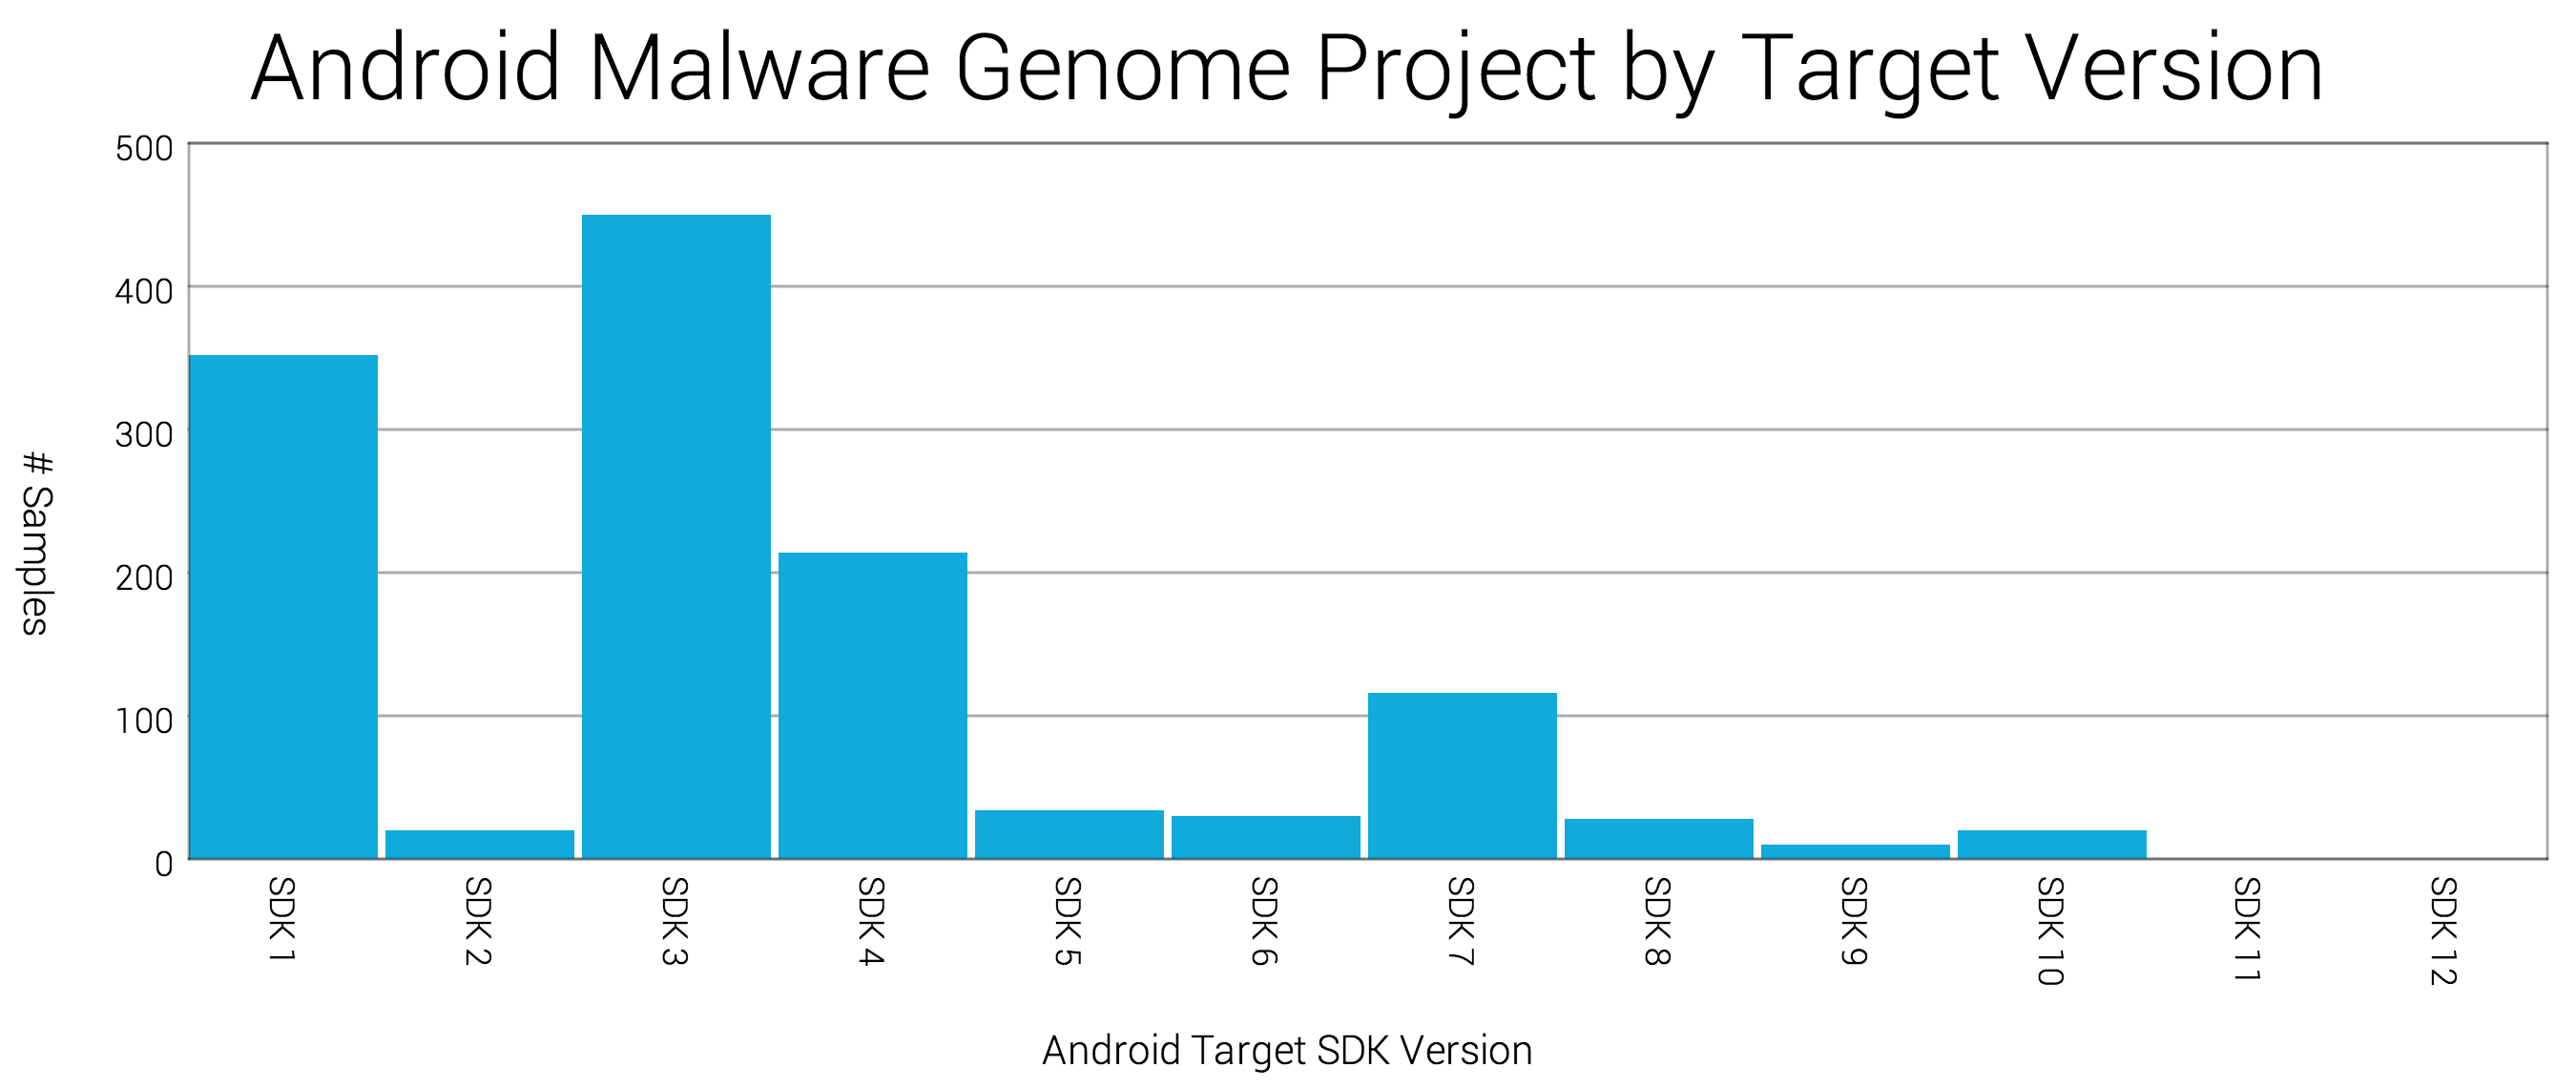
\includegraphics[width=1.0\columnwidth]{figs/MalwareAndSDK}
\caption{Malware from the Android Malware Genome Project by Android Version }
\label{fig:malwaresdk}
\end{center}
\end{figure}

Of these four examples, one --- \textit{RogueSPPush} --- sends premium SMS messages, but does not request \textit{Send SMS}, rendering it ineffective. The three remaining samples --- \textit{DogWars}, \textit{GoldDream} and \textit{DroidDreamLight} --- were Info Theft malware. We found \textit{DroidDreamLight} to be less than worthwhile for testing, due to its rather benign nature: the worst action it performs is uploading the device's IMEI to a remote server. Finally, \textit{GoldDream} has botnet capabilities, making it difficult to test, due to the lack of an existing botnet.

The remaining app, \textit{DogWars}, makes a good testing app. Made as a ``hacktivist'' app in protest of an existing app\citep{symantecdogwars}, \textit{DogWars} repackages a game with code to send SMS messages to all contacts on the next boot. The screenshots in Figure \ref{fig:dogwars_visual} show how AndroMEDA clearly identifies when \textit{DogWars} accesses contacts and sends messages, allowing the user to identify it as malware.

\begin{figure}[h]
\begin{center}
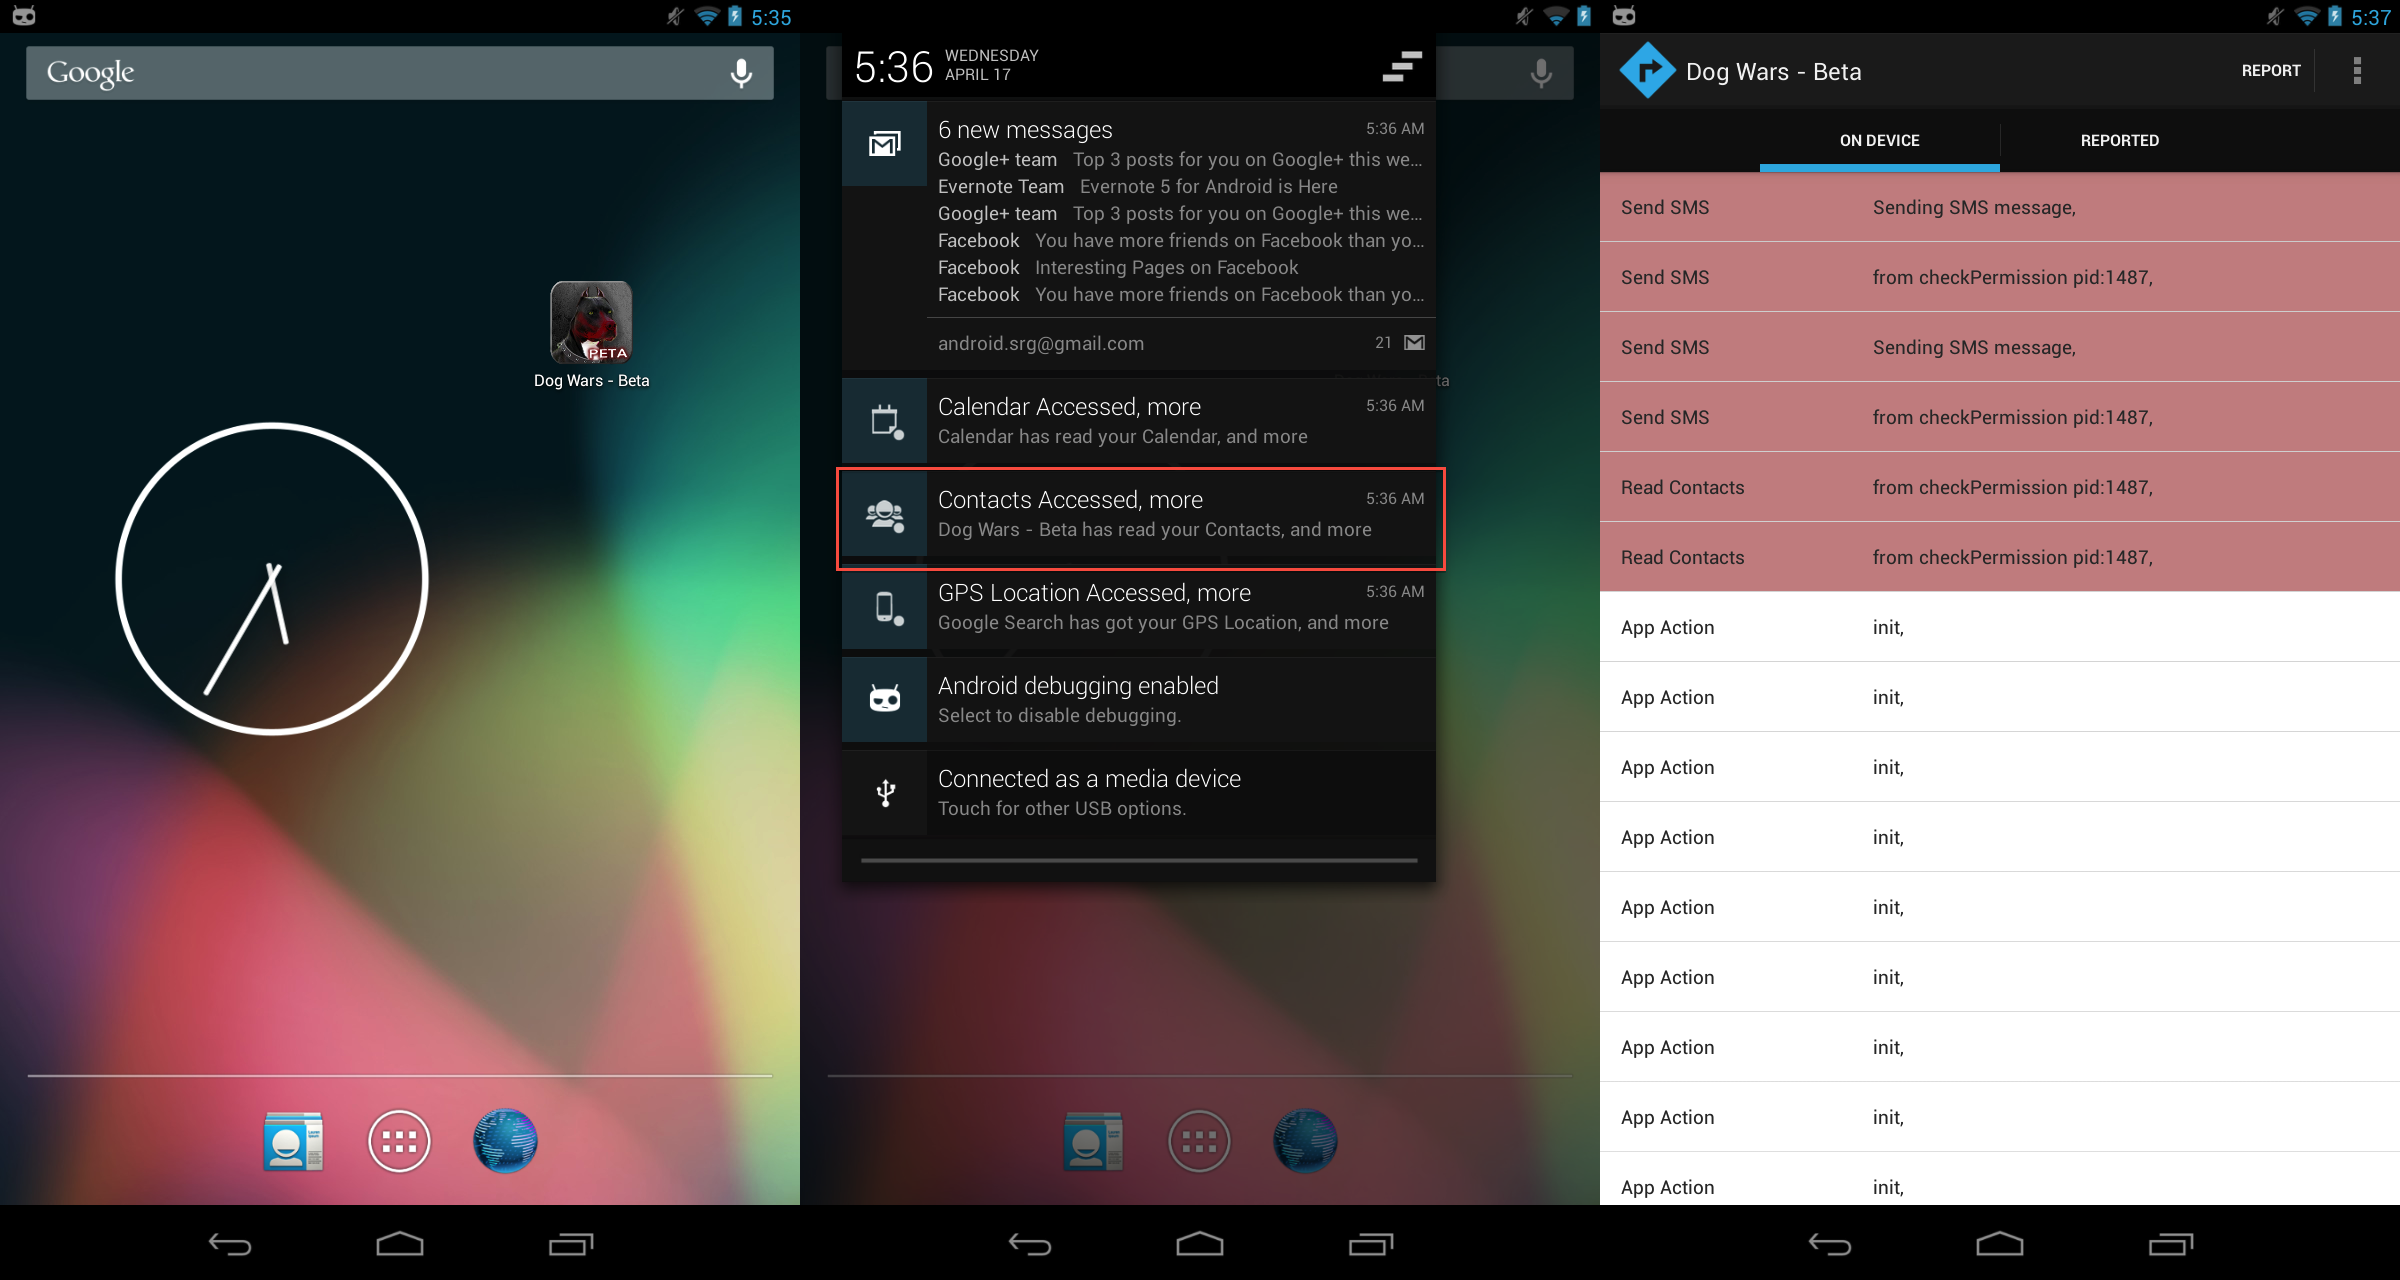
\includegraphics[width=1.0\columnwidth]{figs/dogwars_detection}
\caption{AndroMEDA detecting the \textit{DogWars} Malware (annotated in red) }
\label{fig:dogwars_visual}
\end{center}
\end{figure}

We have demonstrated AndroMEDA's ability to identify malware in existing datasets, but in the process we highlighted the shortcomings of the current Android malware datasets. To test a future-malware oriented framework, it would be ideal to have more sophisticated malware. Rootkits and Premium SMS malware have been addressed by recent versions of Android: so we focus on what we believe to be the future of malware on Android: sophisticated Info Theft Apps. We have defined IncognitoWare as the concept of hiding Info Theft Malware inside of benign apps, designed to silently steal PII and perform other unwanted operations. Since our analysis of Permissions in the GPStore has shown that popular apps tend to request a large amount of PII-related permissions, we can fit them all within the existing Permission Fingerprint. 

\subsection{IncognitoWare Dataset}
\label{sec:incognitoware}
IncognitoWare has recently become one of the most popular forms of mobile malware\citep{nq2013}. FakeInst, discussed in Chapter \ref{sec:premiumsms}, was a repackaged version of Instagram\citep{instagramandroid} that sent premium SMS messages on start. While admittedly basic, more complex versions, such as FakeAngry\citep{fakeangry} have been found, imitating popular games, while in the background stealing PII, installing a rootkit, and joining a botnet.

We introduce a novel set of research IncognitoWare as a representative sample of current and future mobile malware techniques. Our first example sends as much PII as it can find to a remote server; the second silently monitors the phone in the background. We chose not to include a Premium SMS Malware sample, despite its popularity\citep{nq2013}, due to it being addressed in the latest version of Android. By analyzing our framework with this dataset, we hope to demonstrate the effectiveness of addressing the UAA as a main route to detecting malware.

Creating IncognitoWare is straightforward. First, an exploit is designed and coded as its own app. Second, the \textit{apktool}\citep{apktool} utility decompiles any APK file into a set of resources and \textit{smali} files --- decompiled Dalivk bytecode. From there, the \textit{apktool} utility is used again on the exploit, and the \textit{smali} code trees are merged. The exploit entry points are then placed inside of the host app's code, and \textit{apktool} rebuilds the project back into an APK file. This APK is unsigned and requires the malware writer to resign it. This mismatched signature makes the APK unsuitable for uploading to the Google Play Store, but by changing the Android package to something slightly different, it is suitable for deployment in the Google Play Store, or third party markets.


\subsection{Info Theft IncognitoWare}
Our first example of next-generation IncognitoWare is simple: embed PII stealing code into any app, but only execute it after the user has logged in. This act of logging in is sufficient to bypass automated monitoring tools like Google Bouncer. Only executing the code after the user has performed an action also creates a plausible scenario where the situation might have been intended. Ultimately, however, since nothing is presented to the user, such an action is a clear violation of the UAA and is seen as malicious. Furthermore, we stay within the Permission Fingerprint of the original software, meaning it is not only invisible when installing, but blocking the permission outright, or feeding it fuzzed data, would ultimately result in legitimate actions being interfered with. This simple example is powerful enough to steal nearly all highly-valuable PII from a device, yet inconspicuous enough to be undetected, and legitimate enough to be unblocked.

AndroMEDA, however, can easily detect this example, seen in Figure \ref{fig:infotheft_visual}. After the user logs in, AndroMEDA immediately alerts the user that the PII has been read. The user then reviews the data shown in Figure \ref{fig:infotheft_logs_malware} and decides whether or not its actions break the UAA and if the app should be trusted with the actions. By comparison, the logs of the untainted version of the app can be seen in Figure \ref{fig:infotheft_logs_nonmalware}. It is worth noting that the logs in Figure \ref{fig:infotheft_logs_nonmalware} and \ref{fig:infotheft_logs_malware} were not generated by the current companion app, but offline; with additional context added describing what the user was doing at the time of specific actions, and that these visualizations are a focus of future work.

\begin{figure}[h]
\begin{center}
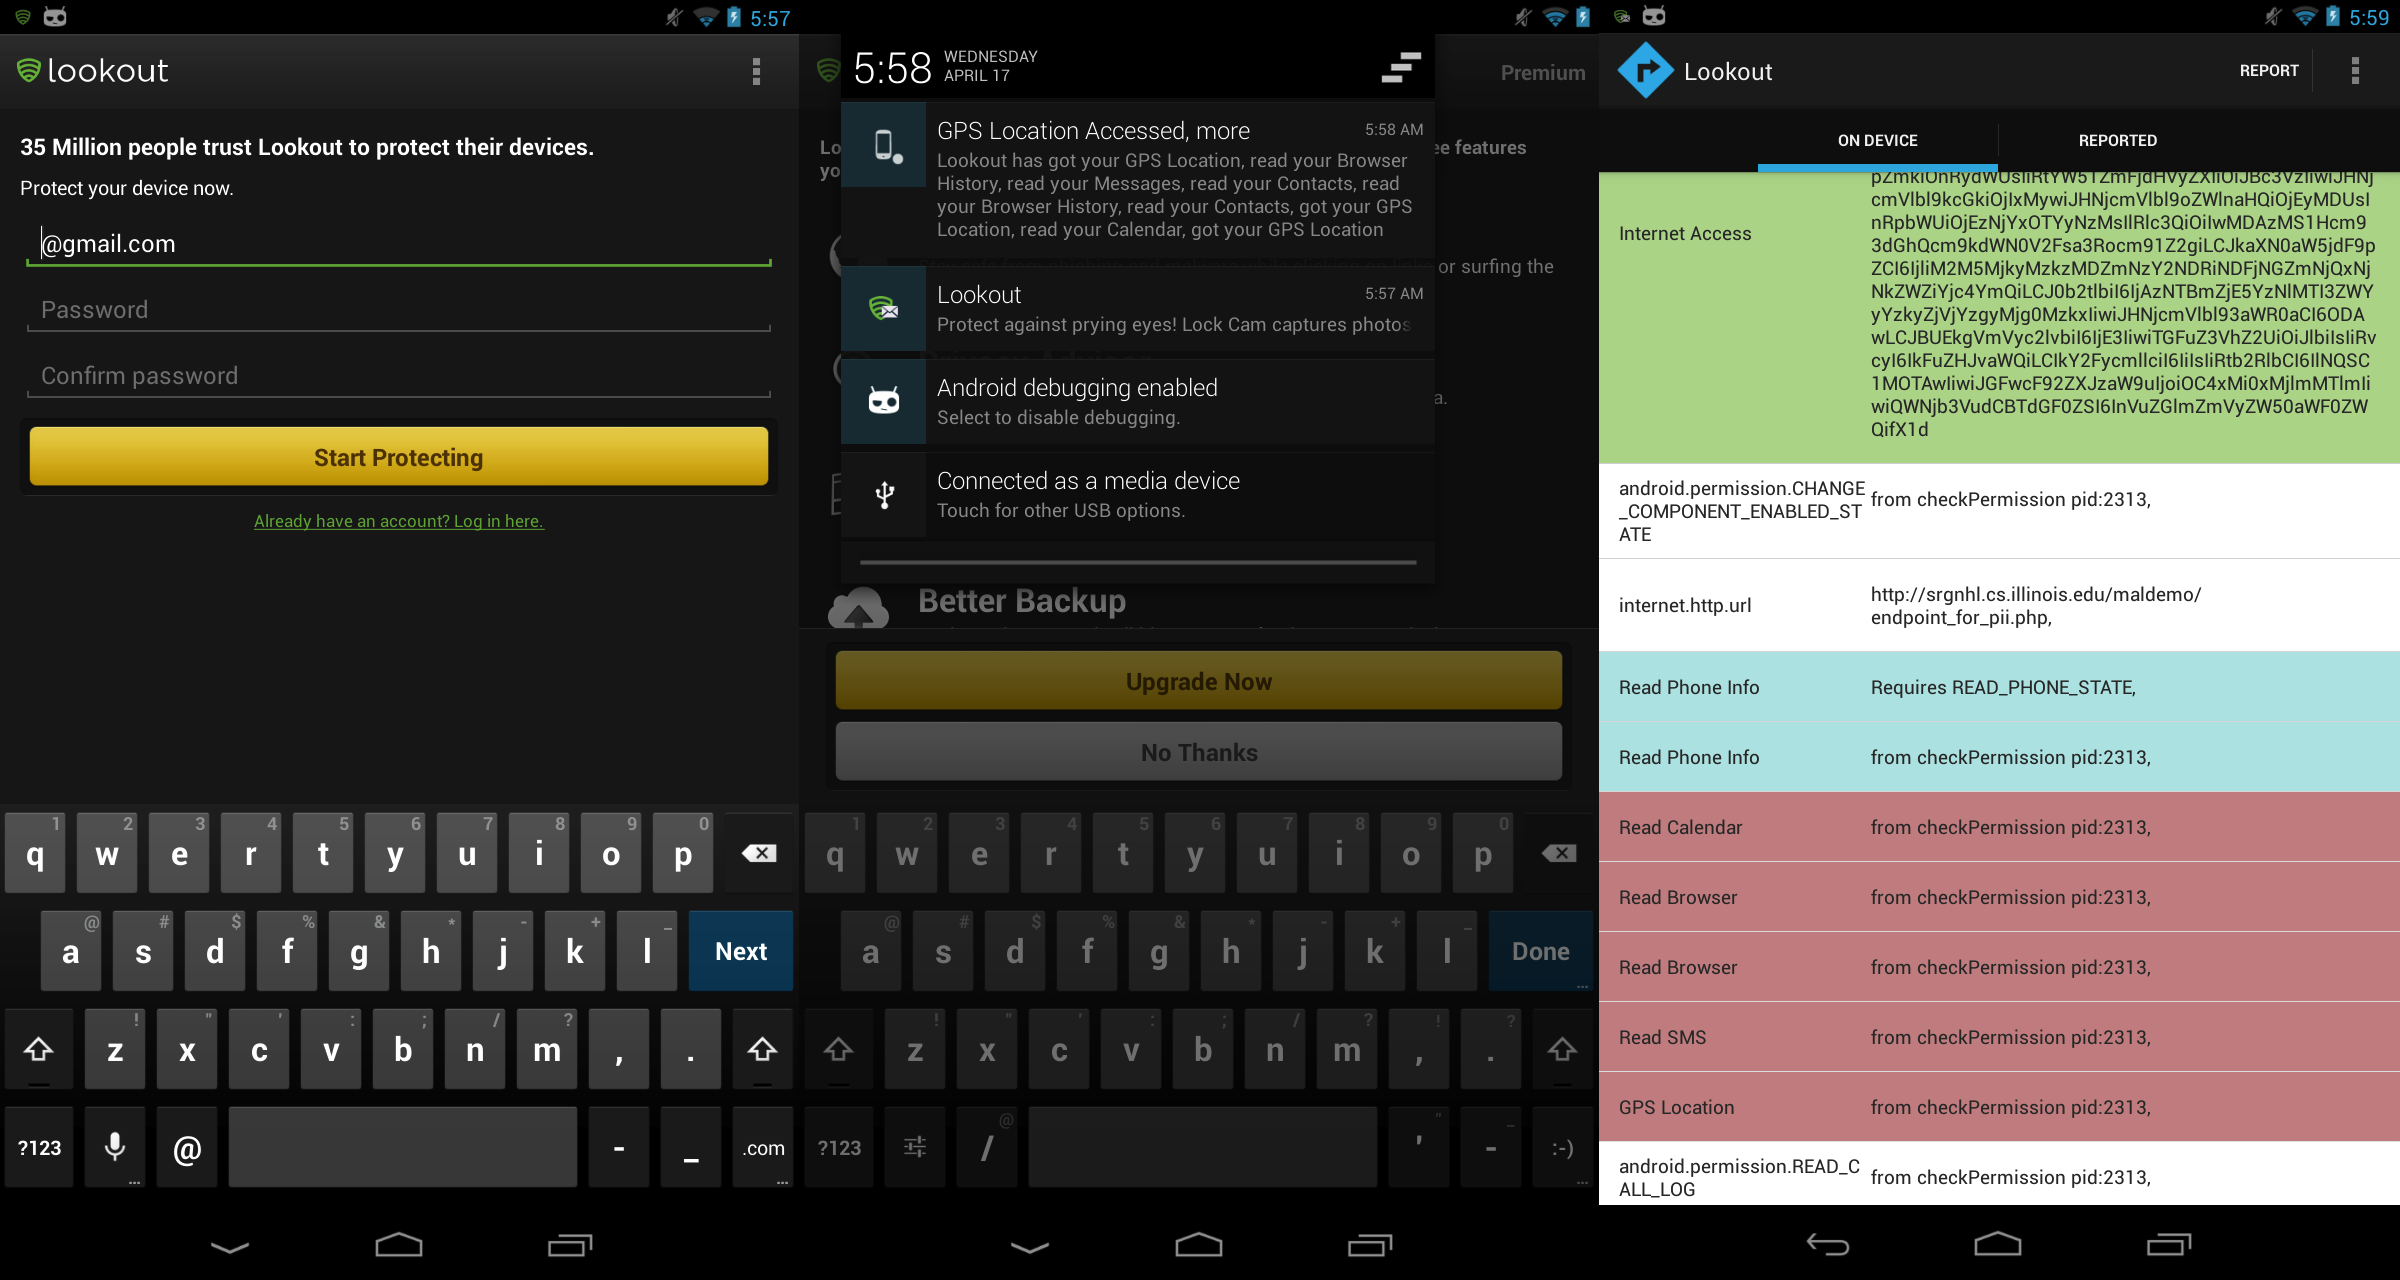
\includegraphics[width=1.0\columnwidth]{figs/lookout_detection}
\caption{AndroMEDA detecting the Info Theft IncognitoWare embedded within a security app }
\label{fig:infotheft_visual}
\end{center}
\end{figure}

\begin{figure}[h]
\begin{center}
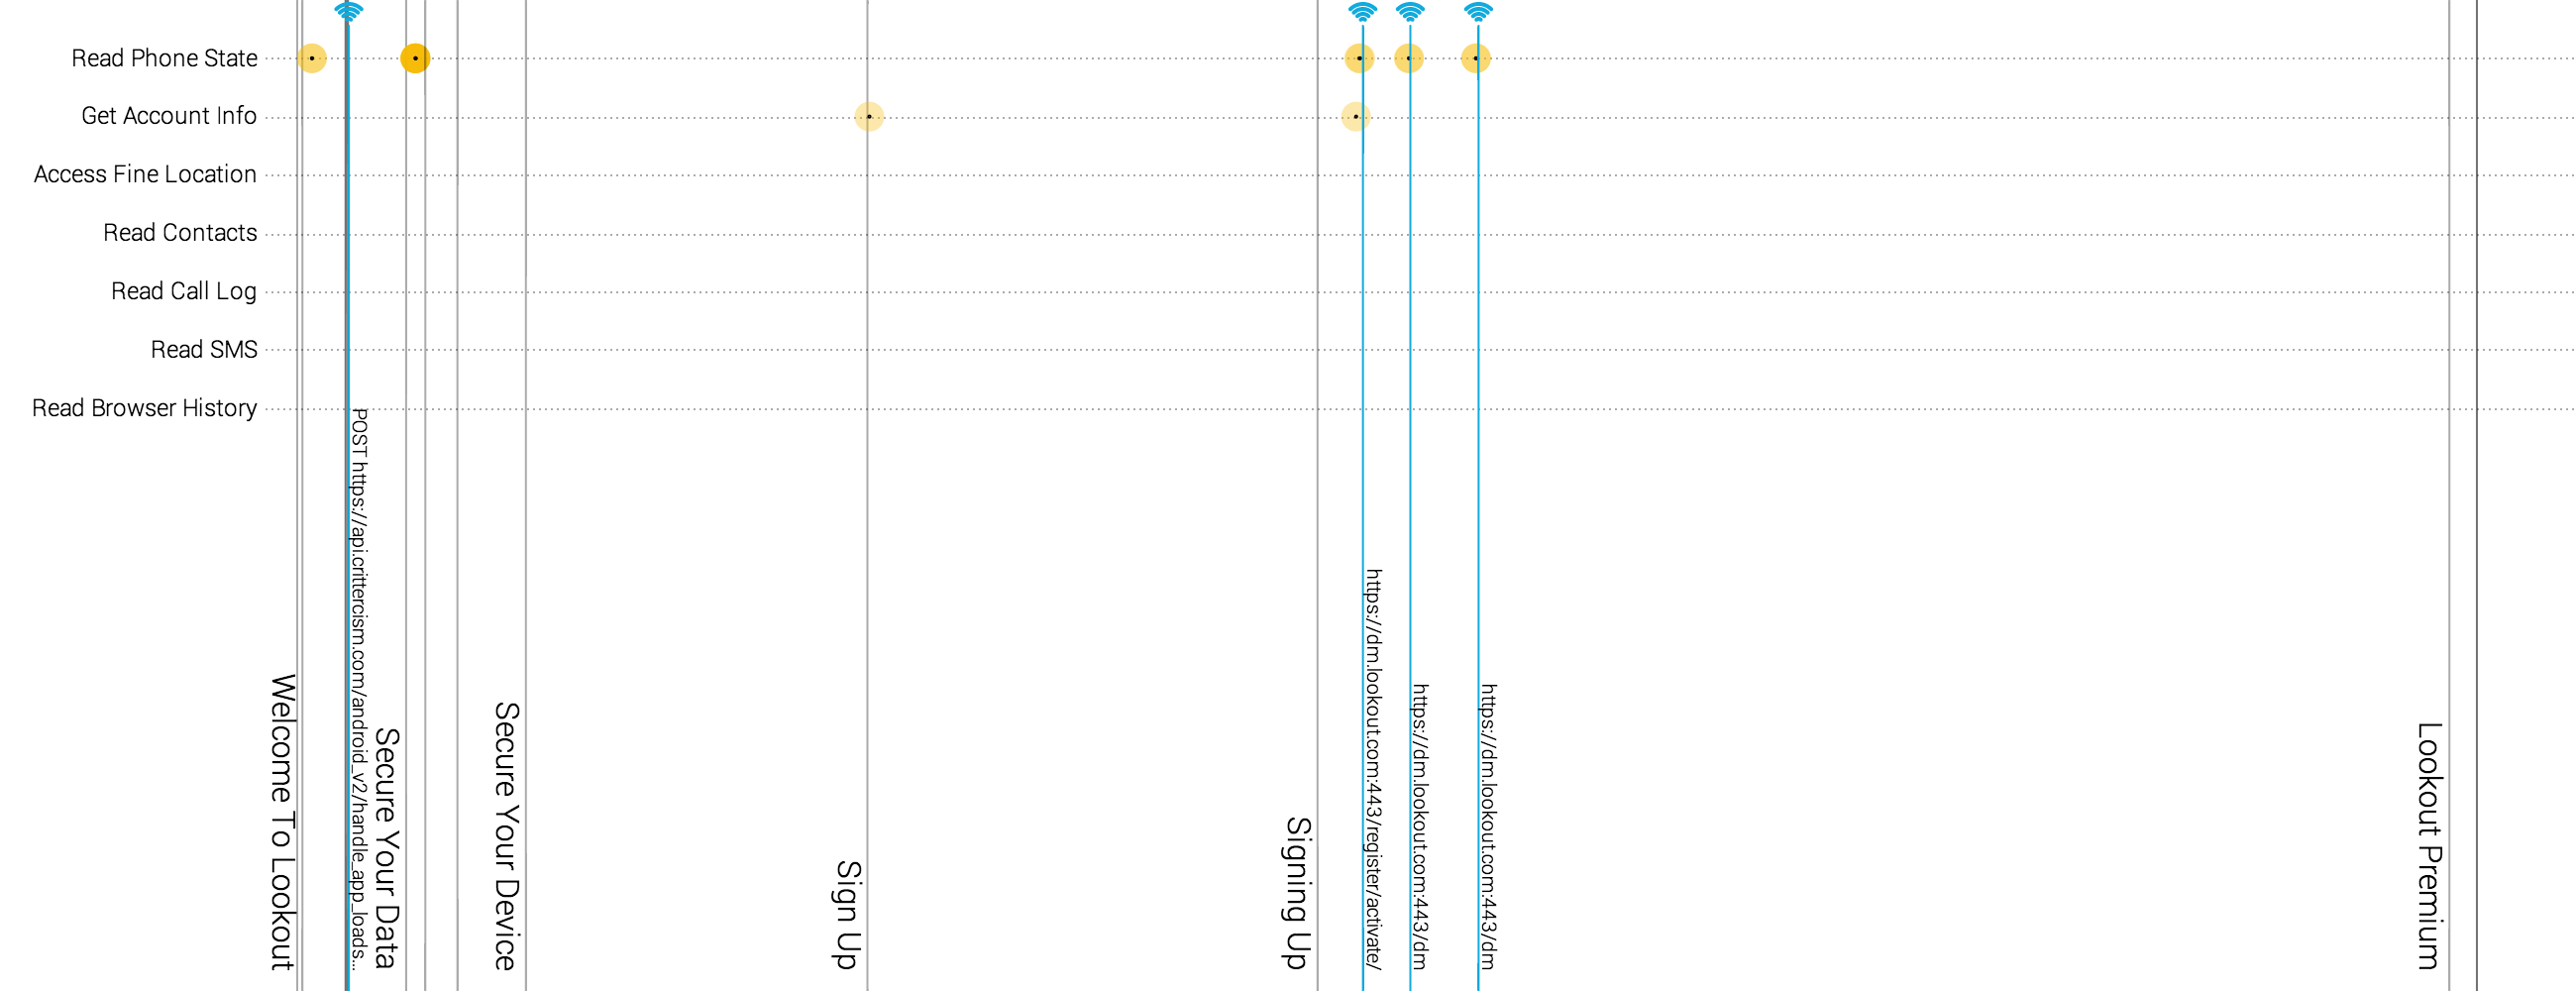
\includegraphics[width=1.0\columnwidth]{figs/AndroMEDA_Lookout_Notmalware}
\caption{AndroMEDA logs of the normal version of the security app }
\label{fig:infotheft_logs_nonmalware}
\end{center}
\end{figure}

\begin{figure}[h]
\begin{center}
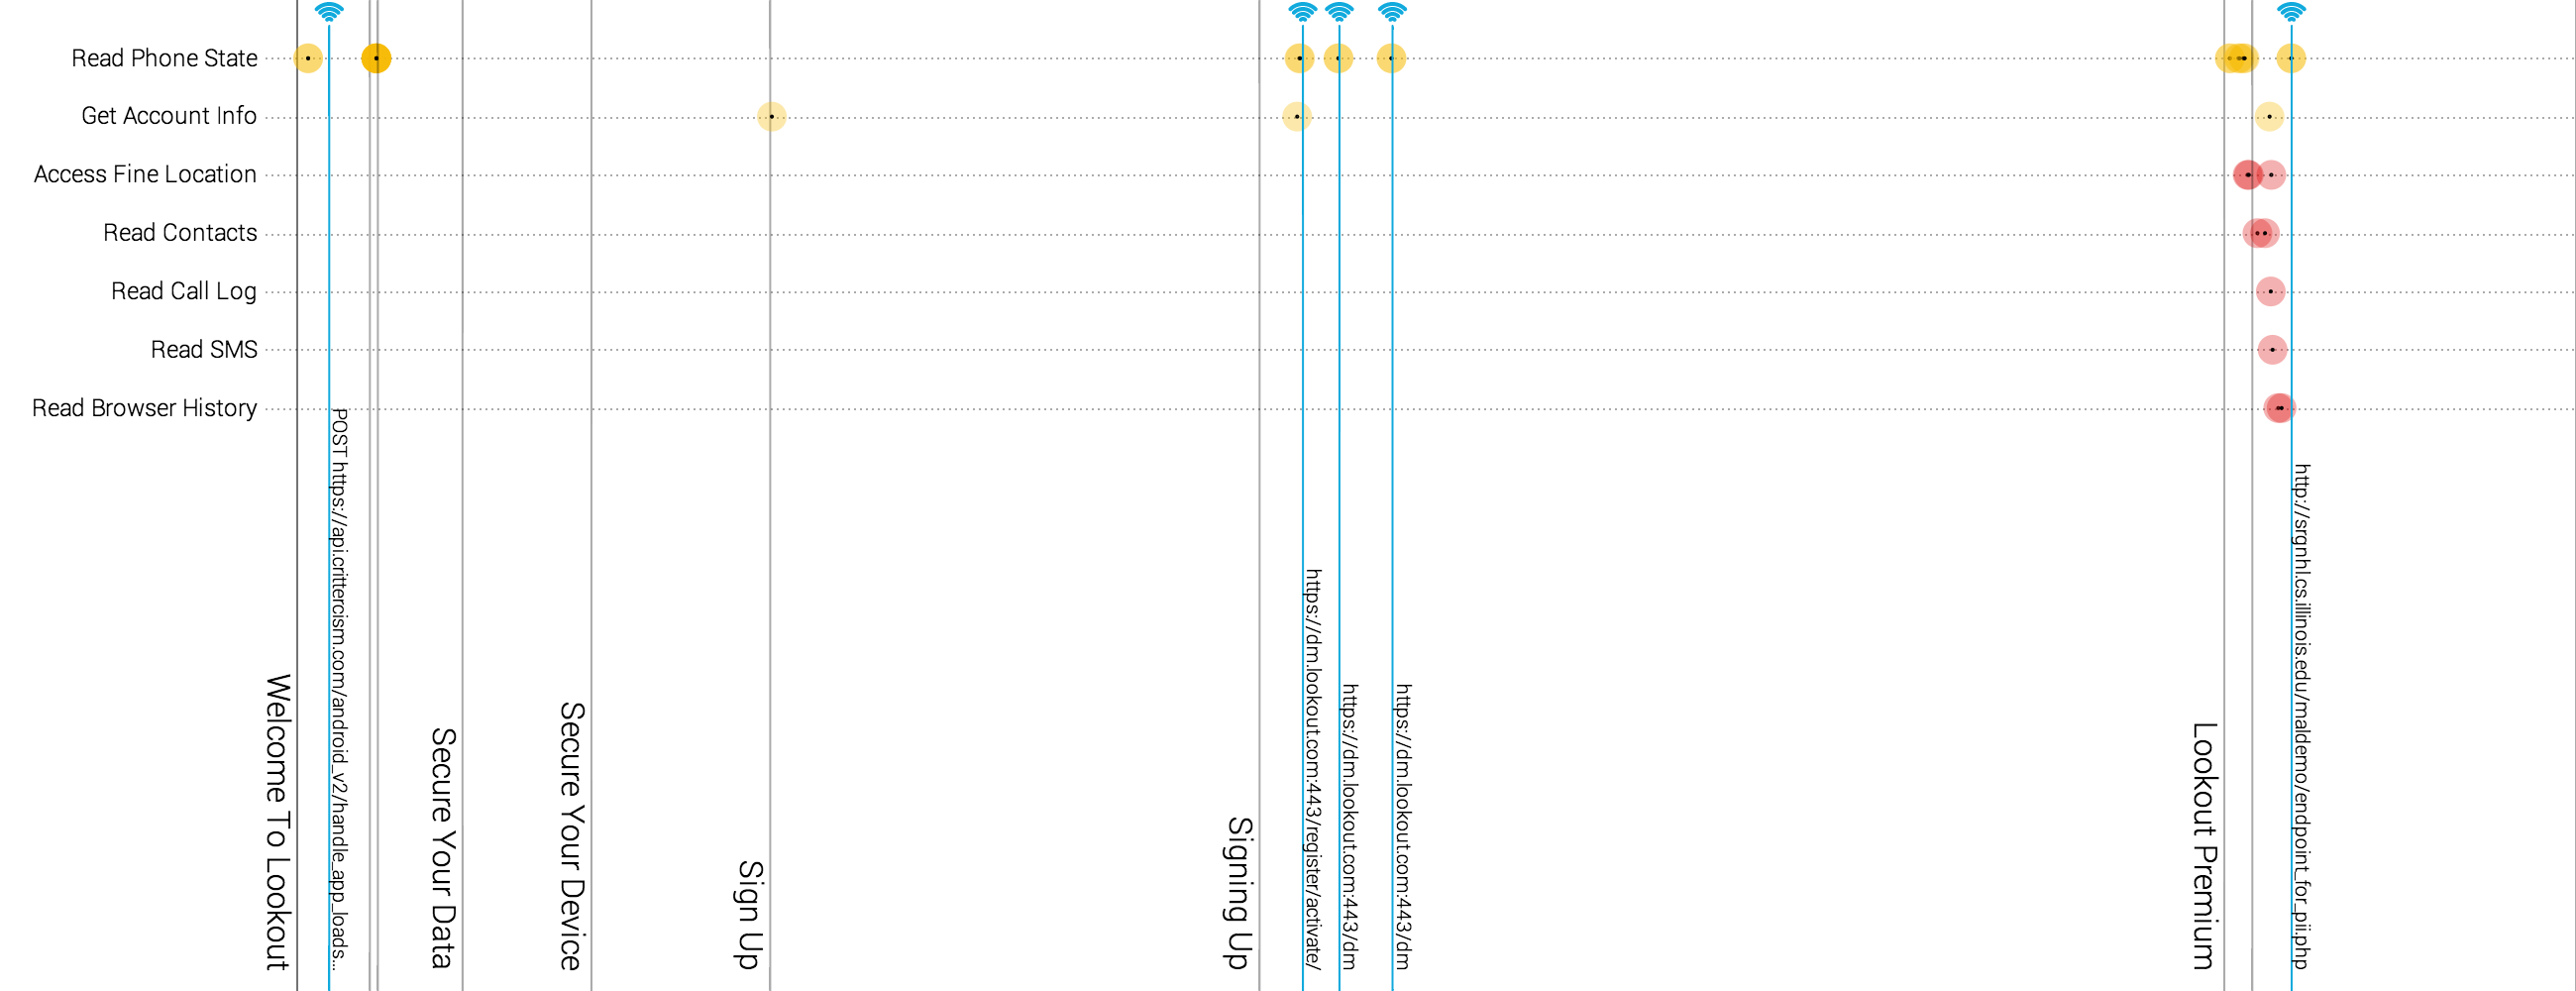
\includegraphics[width=1.0\columnwidth]{figs/AndroMEDA_Lookout_Malware}
\caption{AndroMEDA logs of Info Theft IncognitoWare embedded within a security app }
\label{fig:infotheft_logs_malware}
\end{center}
\end{figure}




\subsection{Spyware IncognitoWare}
Our next example of sophisticated IncognitoWare is designed to continuously spy on the user, while staying within the capabilities of a trusted app. We first find an app that has all the requirements for spyware: access to location, Internet, wake lock, and starting at boot. We then introduce our malware, which is triggered an arbitrary amount of time after the initial startup --- five minutes is long enough to evade Google Bouncer\citep{mansfield2012android}. After that, the device wakes up every five minutes, gathers a location fix, and sends that information to a remote location. As before, many examples exist of apps that use similar behavior for non malicious purposes, making policies to guard against it difficult.

Once again, AndroMEDA can alert the user of this kind of behavior easily. Figure \ref{fig:spyware_visual} shows the user installing the app, starting it up, going to the home screen, and eventually noticing the suspicious behavior when the phone is idling. The user then inspects the logs of this app, (Figure \ref{fig:spyware_logs_malware} --- with context added), finds this to be a continuous occurrence, and decides that the app is malware. Compared to Figure \ref{fig:spyware_logs_nonmalware_noloc}, the app is clearly accessing location in a suspicious pattern --- and the usage pattern is the key indicator. When compared to Figure \ref{fig:spyware_logs_nonmalware_location}, however, the main indicator is the address the information is going towards, an address not associated with the main app. The normal logs in Figure \ref{fig:spyware_logs_nonmalware_location} may break UAA for some users --- the app logs the user's location in the background and sends it to a remote server. Overall, this highlights the ability of AndroMEDA to capture both the context and use of permissions: the patterns of access provide context and the network locations provide use.




\begin{figure}[h]
\begin{center}
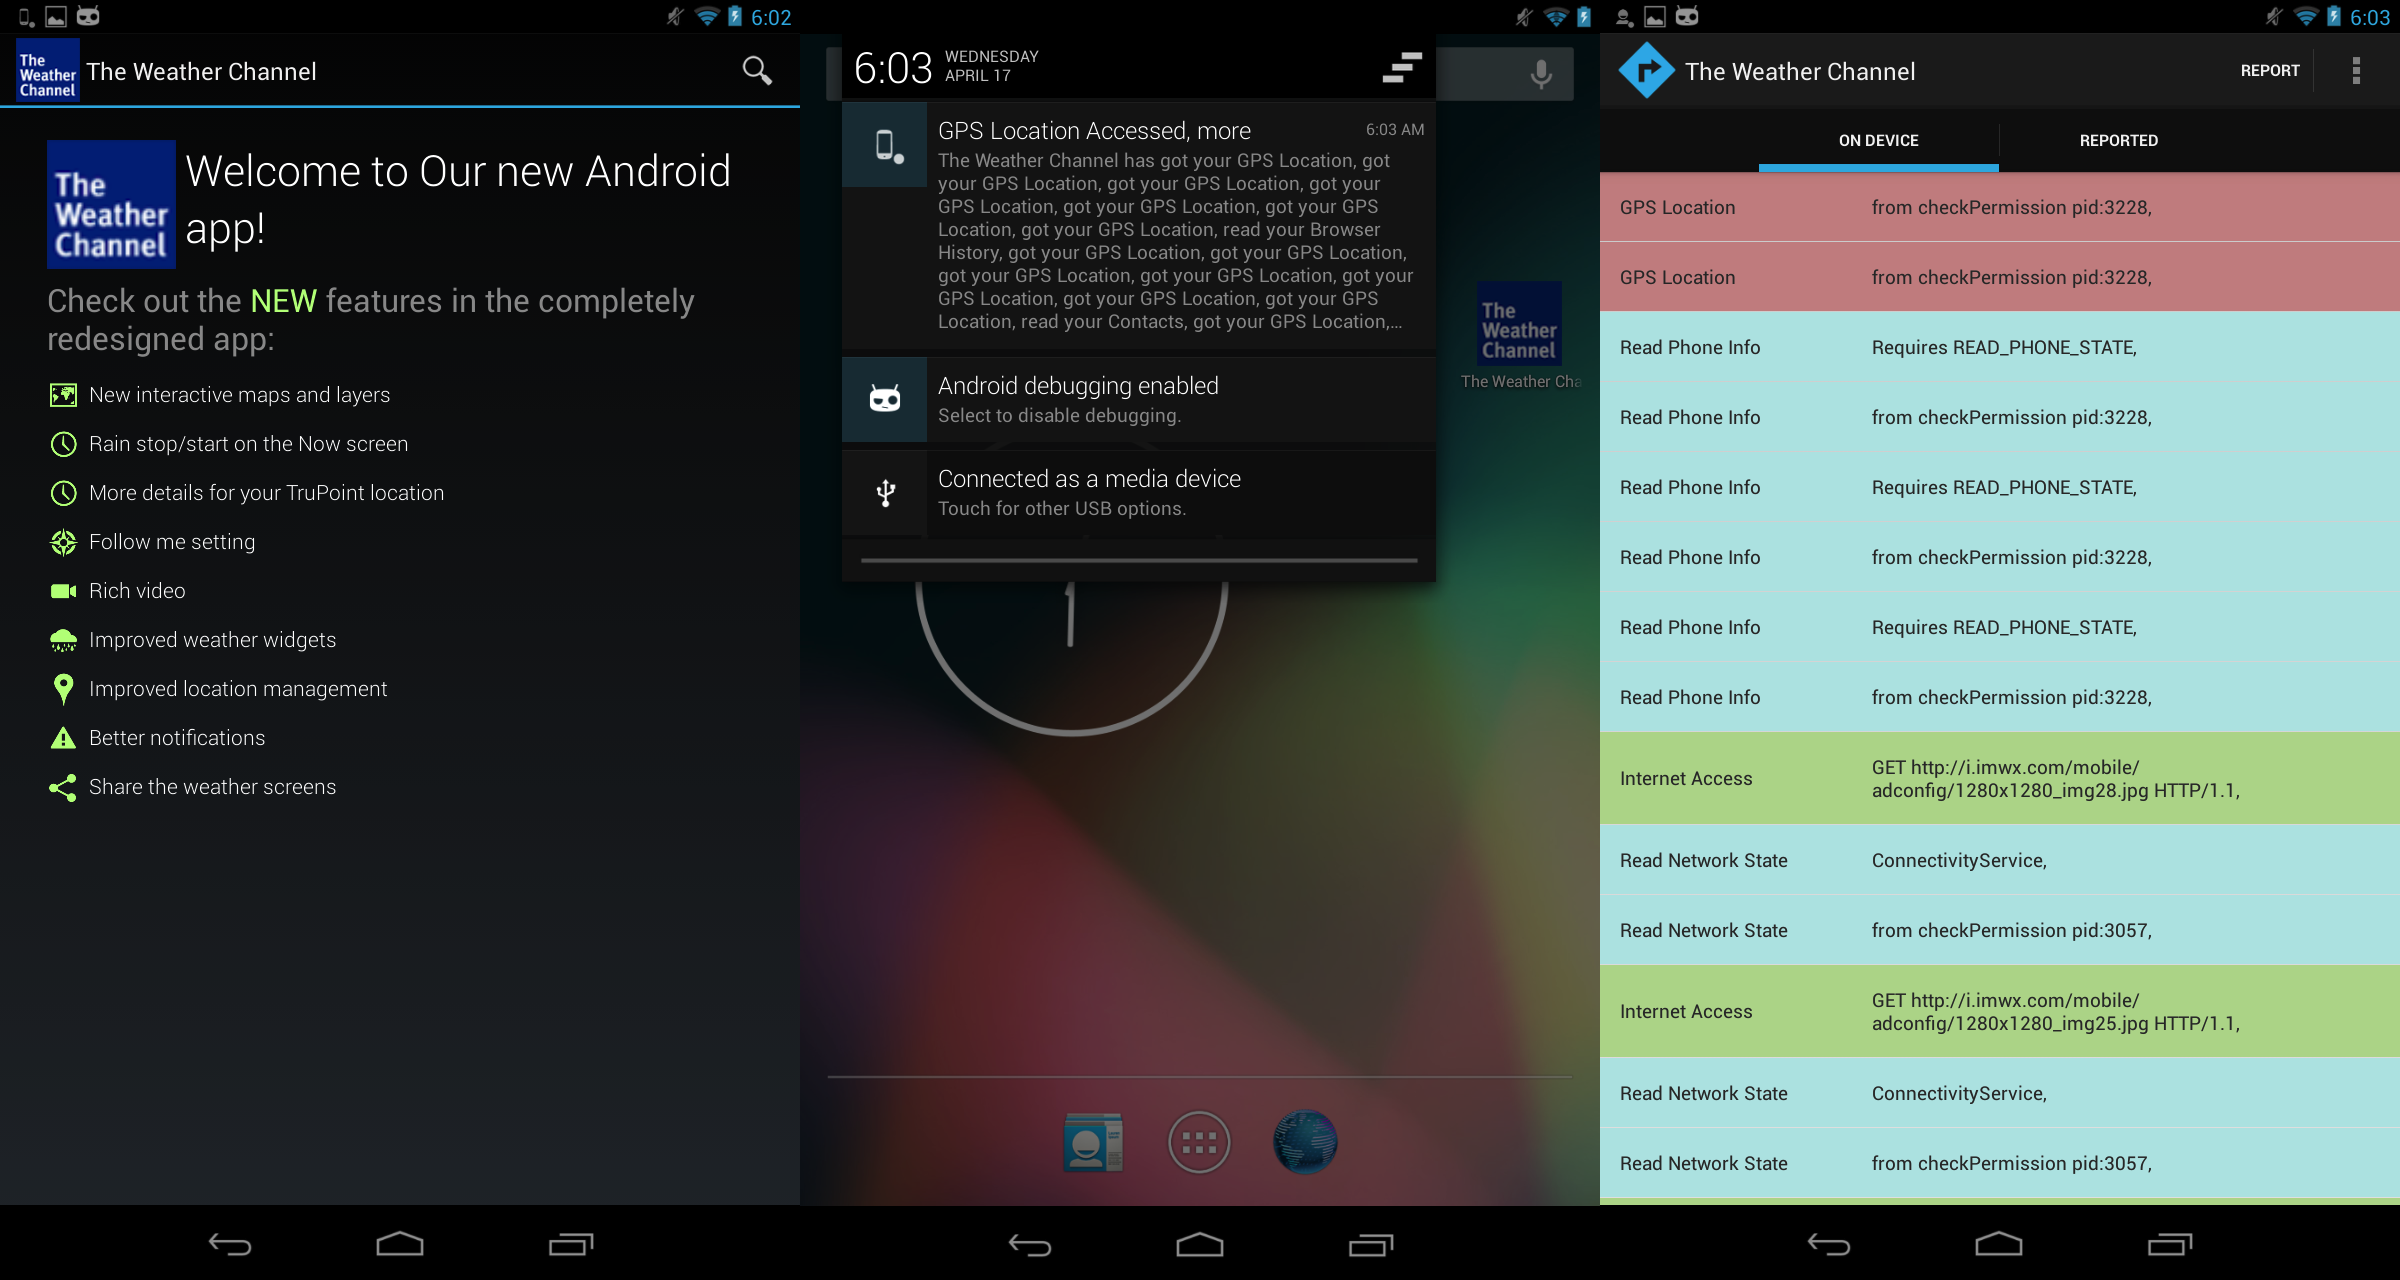
\includegraphics[width=1.0\columnwidth]{figs/weather_detection}
\caption{AndroMEDA detecting the Spyware IncognitoWare embedded within a weather app }
\label{fig:spyware_visual}
\end{center}
\end{figure}


\begin{figure}[h]
\begin{center}
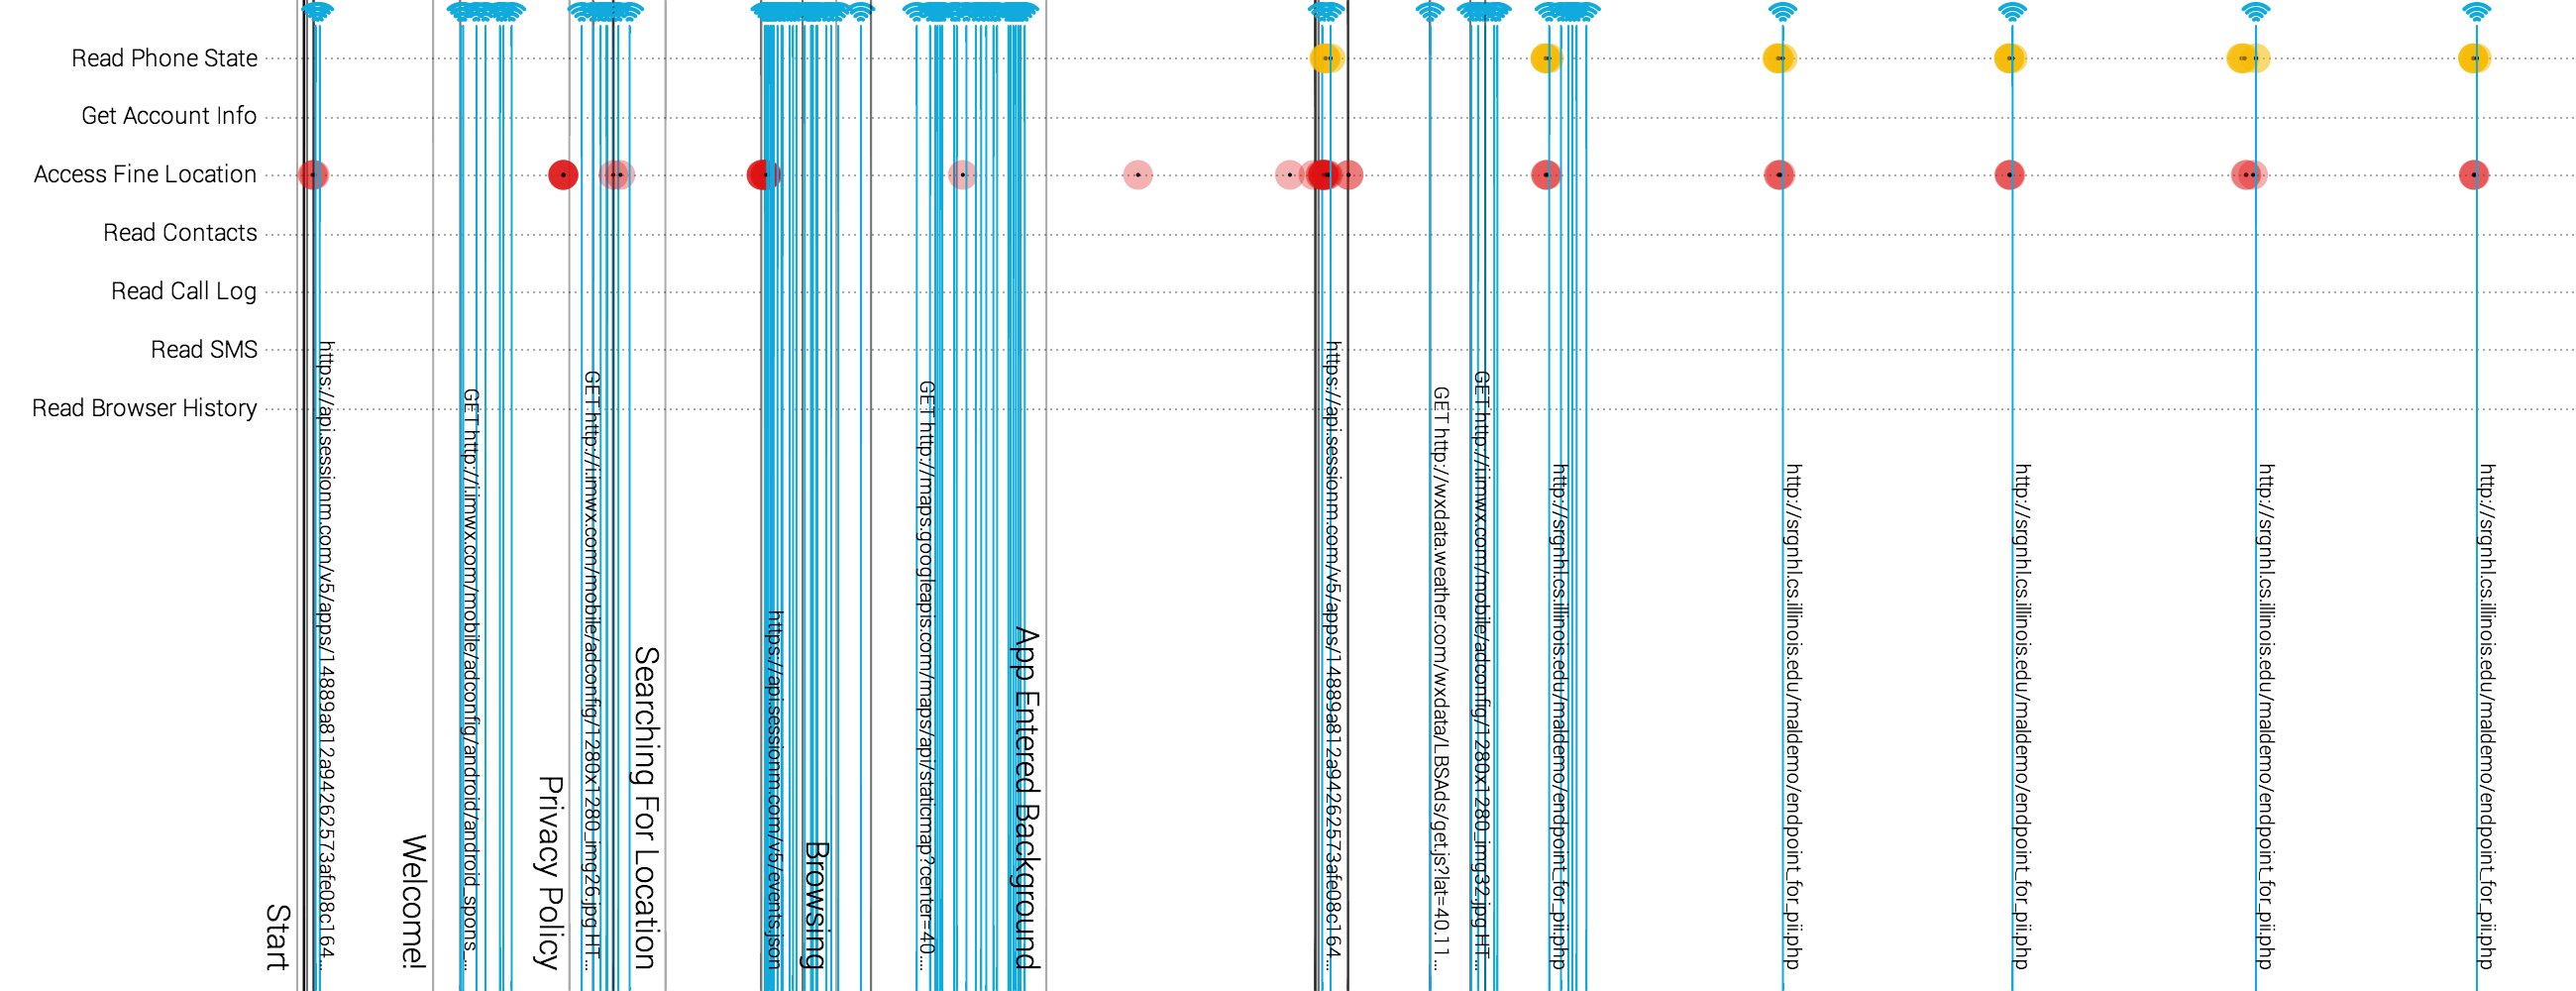
\includegraphics[width=1.0\columnwidth]{figs/AndroMEDA_Weather_Malware}
\caption{AndroMEDA logs of Spyware IncognitoWare embedded within a weather app }
\label{fig:spyware_logs_malware}
\end{center}
\end{figure}

\begin{figure}[h]
\begin{center}
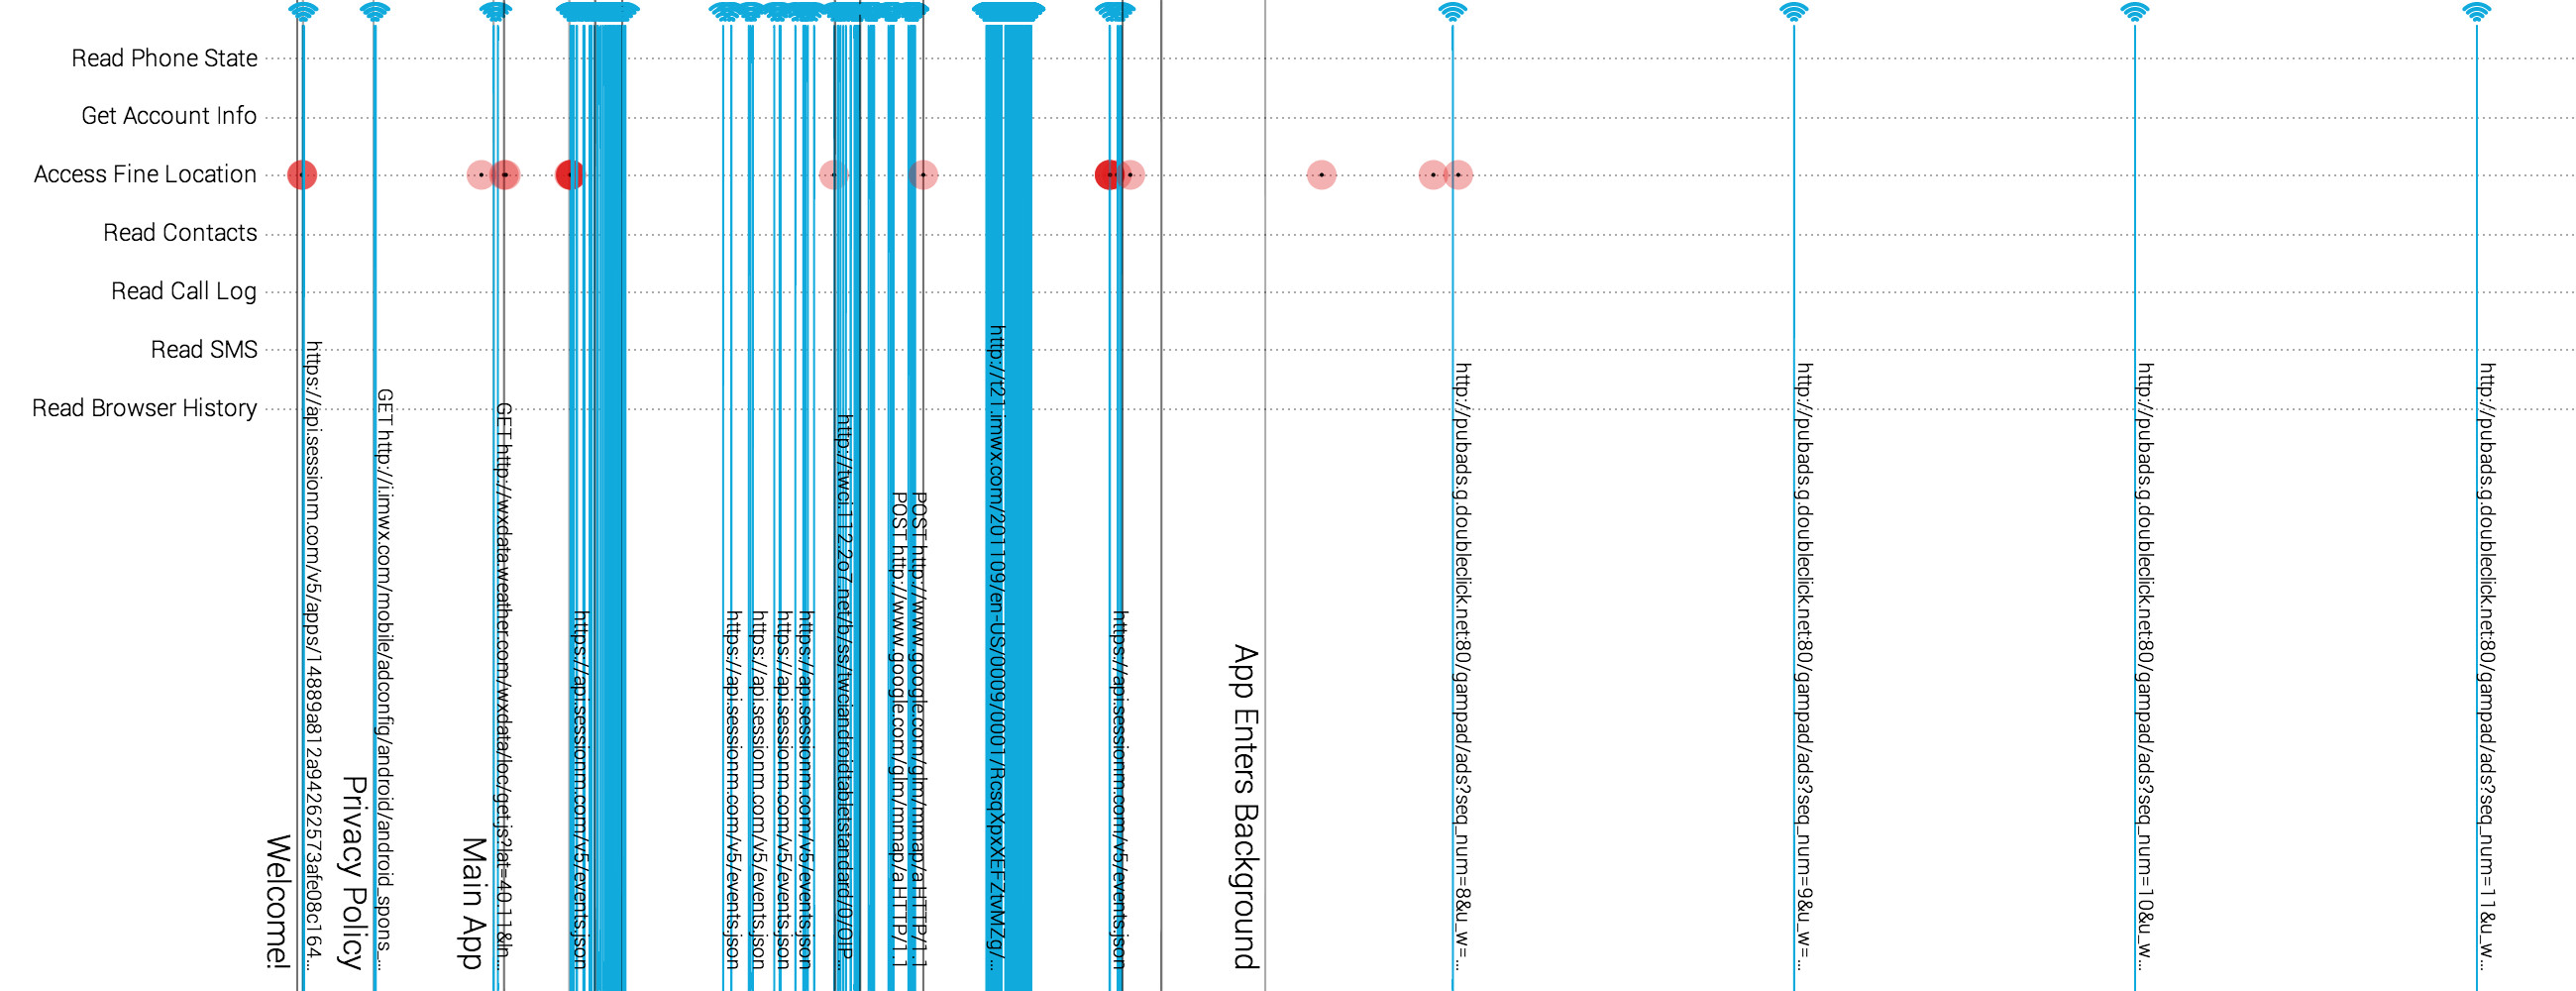
\includegraphics[width=1.0\columnwidth]{figs/AndroMEDA_Weather_Notmalware_Location}
\caption{AndroMEDA logs of a normal version of a weather app, when the user has consented to location gathering }
\label{fig:spyware_logs_nonmalware_location}
\end{center}
\end{figure}


\begin{figure}[h]
\begin{center}
\includegraphics[width=1.0\columnwidth]{figs/AndroMEDA_Weather_Notmalware_Nolocation}
\caption{AndroMEDA logs of a normal version of a weather app, when the user has not consented to location gathering }
\label{fig:spyware_logs_nonmalware_noloc}
\end{center}
\end{figure}


\subsection{Companion App}
When the user reviews the logs, they have the option to report suspicious behavior, giving a description of what the user was doing and what the suspicious behavior was. These reports are collected in a centralized database. The companion app also listens for when the user installs new applications and checks the same database to see if there are any existing reports. If the number of reports passes a threshold, the companion app will notify the user, enabling them to review what other people have reported about the apps. These features --- being notified of suspicious apps and reviewing them --- does not require the AndroMEDA extensions and can be installed on any Android device. This enables a small set of users to alert a much larger population.

\subsection{Conclusion}
Overall, we have demonstrated that the ability to log and visualize app behavior can lead to an increased ability to detect malware. Our logs and visualizations show clear differences between actions that fall within the User-App Agreement and actions that do not, even being able to visualize actions that may break some user's UAA but not others. The ability to report when an app breaks the UAA and having that report spread to other users enables AndroMEDA to become a community effort, further increasing its effectiveness.






































\section{Conclusion}
\label{sec:conclusion}
AndroMEDA helps users understand the context in which their Personally Identifiable Information is used, which allows them to make more informed decisions on whether an app is acting maliciously or not. In this paper, we introduced four key items: User-App Agreement, Android Census, AndroMEDA and IncognitoWare.

\subsubsection{User-App Agreement}
%We analyze the state of Android and Permissions, and conclude the need to address the User-App Agreement, which is a framework for consenting and trusting specific actions an app may take. It lies at the heart of classifying Info Theft Malware. Android Permissions address the capabilities of an app, but fail to address the context and use of those capabilities, which are crucial to trusting an app's actions.

We analyzed the current Android security framework: the Permission System, and found its main flaws were its lack of addressing context and use, which we generalized into the User-App Agreement --- a framework for consenting to and trusting specific actions an app may perform. Whereas Android Permissions exceeded at defining general capabilities of an app, and these capabilities further shape the User-App Agreement, they fail to address the context in which the permissions are used and what they are used for.

\subsubsection{Android Census}
To perform a full analysis of the current state of Android Permissions, we use a novel dataset, Android Census. By analyzing more than 80\% of apps in the Google Play Store, we are able to better understand the interrelationship of permissions and expected behavior. We produce key insights as to the popularity of apps versus their PII permissions and when apps deviate from their expected behavior, potentially violating the User-App Agreement. We then analyze a comprehensive malware dataset using the same techniques and find that many types of malware can be identified purely by its Permission Fingerprint. We conclusively show the connection between Permissions and Expected Behavior is present, but not strong enough to differentiate between Info Theft Malware and many popular apps.

\subsubsection{AndroMEDA}
Building off the concept of the User-App Agreement, we introduce AndroMEDA. Key parts of the User-App Agreement were previously unavailable to the user until AndroMEDA. By giving the user more information on the context and use of permissions, they can evaluate whether or not they trust those actions and, ultimately, whether or not the app is acting maliciously or not. After untrusted behavior is spotted, the actions can be reported, and knowledge can be spread to all users. All of this increases user's awareness of app behavior and helps mitigate Info Theft Malware on Android.

\subsubsection{IncognitoWare}
We highlighted the need for more modern Android malware datasets. To address this, we introduced a dataset of IncognitoWare --- repackaged trusted apps with additional malicious behavior embedded. We believe this is a more comprehensive look at Android security because it highlights the need to understand context in order to identify malicious behavior.

\subsection{Future Work}
\label{sec:futurework}
AndroMEDA is, ultimately, not a complete solution for detecting all Android malware. Projects like TaintDroid and TISSA provide functionality that would greatly enhance the data gathering abilities and response options of AndroMEDA. Integrating TISSA would allow users or the AndroMEDA system to temporally block access to sensitive data, while unblocking access to the same data at a later time when the user trusts the action. Overall, adding more API instrumenting would prove useful, as projects like TapLogger provide future challenges.

A main focus of AndroMEDA is providing feedback to the user; to that end, visualization is an important area of future work. Visualizing the wealth of information in a concise way that avoids user fatigue is a main challenge and subject to future study.

AndroMEDA could also benefit greatly from the probabilistic modeling of pBMDs and Crowdroid, in correlating user action with permission behavior. These would not replace the need to alert the user, but would instead be better able to dictate when to send different classes of alerts to the user --- as the decision of what is malware is ultimately up to them.

The wealth of data in Android Census was also not fully explored. We are currently interested in seeing if specific keywords in user reviews correlate with malicious software or other problematic apps. Many more areas of metadata --- like the description, developer, etc --- can be further explored, to see if it gives additional insight into the nature of malware on Android.

Finally, the concept of the User-App Agreement introduced in this paper could be greatly expanded upon. User Studies of trust in specific actions can greatly increase our understanding of what actions users tend to trust and when they are untrustworthy. These same user studies could also help demonstrate the effectiveness of AndroMEDA in spotting Info Theft Malware.

























\section{Future Work}
THE FUTURE.























\section{Acknowledgments}

%
% The following two commands are all you need in the
% initial runs of your .tex file to
% produce the bibliography for the citations in your paper.
\bibliographystyle{abbrv}
\bibliography{ref}
% You must have a proper ".bib" file
%  and remember to run:
% latex bibtex latex latex
% to resolve all references
%
% ACM needs 'a single self-contained file'!
%
%APPENDICES are optional
%\balancecolumns
\appendix
%Appendix A
\balancecolumns
% That's all folks!
\end{document}
